%%%%%%%%%%%%%%%%%%%%%%%%%%%%%%%%%%%%%%%%%
% 8/22 _3suW10W
% 8/28 _3suW11T
% 8/29 _3suW11W

\documentclass[letterpaper]{article}
\usepackage[paperwidth=8.5in, paperheight=11in]{geometry}
\linespread{1.0}
\normalsize

\usepackage[utf8]{inputenc}

\usepackage{indentfirst}
\usepackage[utf8]{inputenc}
\usepackage{geometry}

\usepackage{amsmath,amsfonts,amsthm} % Math packages
\newcommand{\thickhat}[1]{\mathbf{\hat{\text{$#1$}}}}
\newcommand{\thickbar}[1]{\mathbf{\bar{\text{$#1$}}}}
\newcommand{\thicktilde}[1]{\mathbf{\tilde{\text{$#1$}}}}

\usepackage[english]{babel}
\usepackage[autostyle]{csquotes}

%\usepackage{spverbatim}

\usepackage{listings}
\usepackage{lstautogobble}

\lstset{basicstyle=\ttfamily,
	mathescape=true,
	escapeinside=||,
	autogobble,
	xleftmargin=0.7in,
	xrightmargin=.25in}

\usepackage{graphicx}

\usepackage[export]{adjustbox}

\usepackage{amsfonts} % if you want blackboard bold symbols e.g. for real numbers

\usepackage{amsmath}
\usepackage{chngcntr}
\usepackage{wrapfig}
\usepackage{caption}
\usepackage{subcaption}

%\usepackage{subfig}




\numberwithin{equation}{section} % Number equations within sections (i.e. 1.1, 1.2, 2.1, 2.2 instead of 1, 2, 3, 4)
\numberwithin{figure}{section} % Number figures within sections (i.e. 1.1, 1.2, 2.1, 2.2 instead of 1, 2, 3, 4)
\numberwithin{table}{section} % Number tables within sections (i.e. 1.1, 1.2, 2.1, 2.2 instead of 1, 2, 3, 4)

\title{	
	\normalfont \normalsize 
	\huge The Convergence of IDLA to a Circle \\ % The assignment title
}

\author{Jean-Luc Thiffeault and Ruojun Wang} % Your name

\date{\normalsize\today} % Today's date or a custom date

\begin{document}
	
\maketitle % Print the title
	

\section{An IDLA Simulation and the Boundary}

\subsection{An IDLA Simulation with N Particles}

Internal diffusion-limited aggregation (IDLA) is (?) a cluster growth process in which particles start at one or more sources within a cluster, diffuse outward, and are added to the cluster at the first site outside it they reach. (refer?) 

\subsubsection{Particles move in 8 directions}
I started from  MATLAB codes given by Professor Thiffeault. To beign, we prepare a grid quadrant where the particles can perform the IDLA process:

\begin{lstlisting}
    Ngrid = ceil(1.2*sqrt(Npart)); 
	grid0 = Ngrid+1;                
	grid = zeros(2*Ngrid+1);
	x = -Ngrid:Ngrid;
\end{lstlisting}

%\begin{spverbatim}

%\end{spverbatim}

\noindent
where \texttt{Npart} represents the total number of particles that take part into the simulation. \texttt{Ngrid} represents the length of one side of grid quadrant. We let \texttt{grid0} be the center of the grid quadrant and generate an array with size \texttt{2*Ngrid+1}; a \texttt{Ngrid*Ngrid} grid quadrant is then set up. Core codes to simulate IDLA process are as following: 

\begin{lstlisting}
    drift = [0 0];
    for i = 1:Npart
	  X = [0 0];
      while 1
	    X = X + (randi(3,1,2)-2) + drift;	    
	    if ~grid(X(1)+grid0,X(2)+grid0)
	      grid(X(1)+grid0,X(2)+grid0) = 1;
	      break
        ...
\end{lstlisting}

\noindent
In this for loop, we start the first particle from the location \texttt{X = [0 0]}, which would locate at the center \texttt{grid0} of the quadrant we set previously. Then inside the while loop generates the coordinate that the next particle would locate. As the definition of IDLA process states, the next particle would move due to a random direction realized by \texttt{(randi(3,1,2)-2)}. A drift \texttt{drift} might be added to effect the final shape of the particles could form; the direction of drift can be given by \texttt{drift = [0 0]} before the for loop. The codes in if statement just says the particle would keep moving due to \texttt{(randi(3,1,2)-2)} until it finds an unoccupied grid to settle down. An occupied grid would be marked as "1" then. In this first simulation, we want the particles to move in 8 directions randomly (i.e. up, down, left, right, upper left, upper right, lower left, lower right). The results of the simulation are shown in Fig.1.1. We can observe that with the growth of the number of particles which participate in the IDLA process, the boundary of the shape tends to be circular, and hence such a convergence to a circle intrigues us to do further study.

\begin{figure}[htbp]
	\centering
	\begin{subfigure}[b]{0.3\textwidth}
		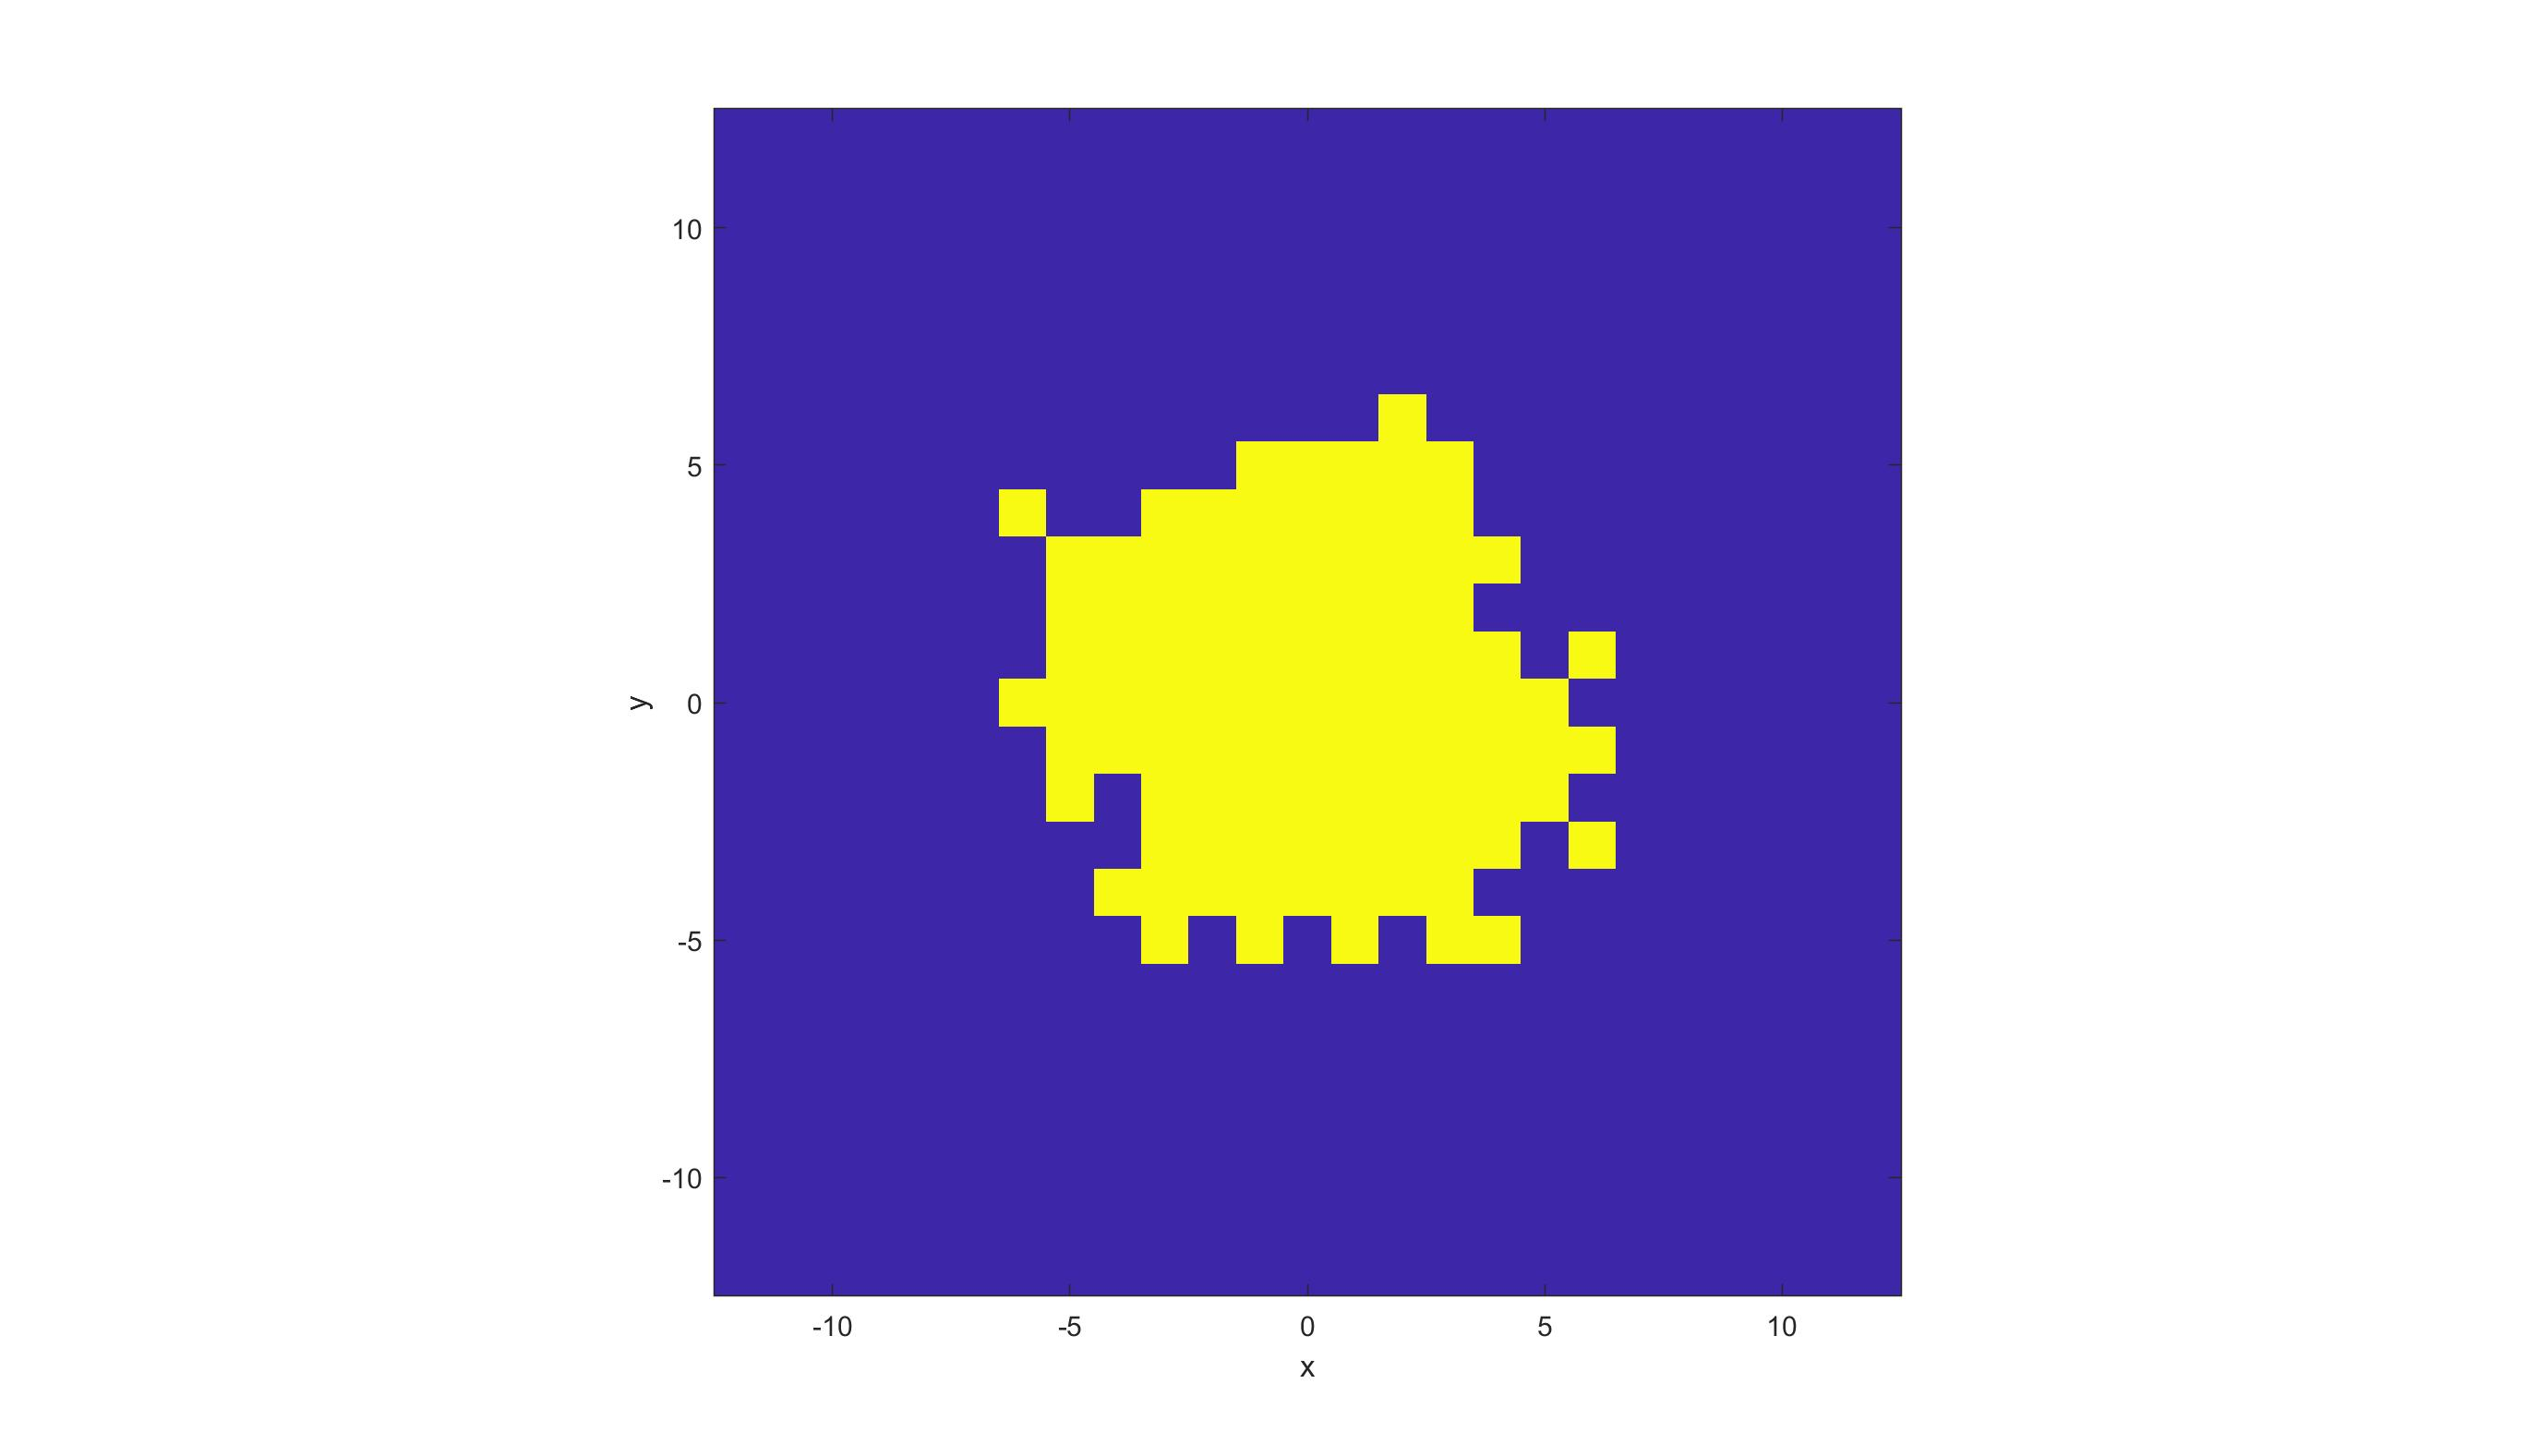
\includegraphics[width=\textwidth]{8direct_Npart100_3suW11T}
		\caption{\texttt{Npart = 100}}
		\label{8direct_Npart100_3suW11T}
	\end{subfigure}
	\begin{subfigure}[b]{0.3\textwidth}
		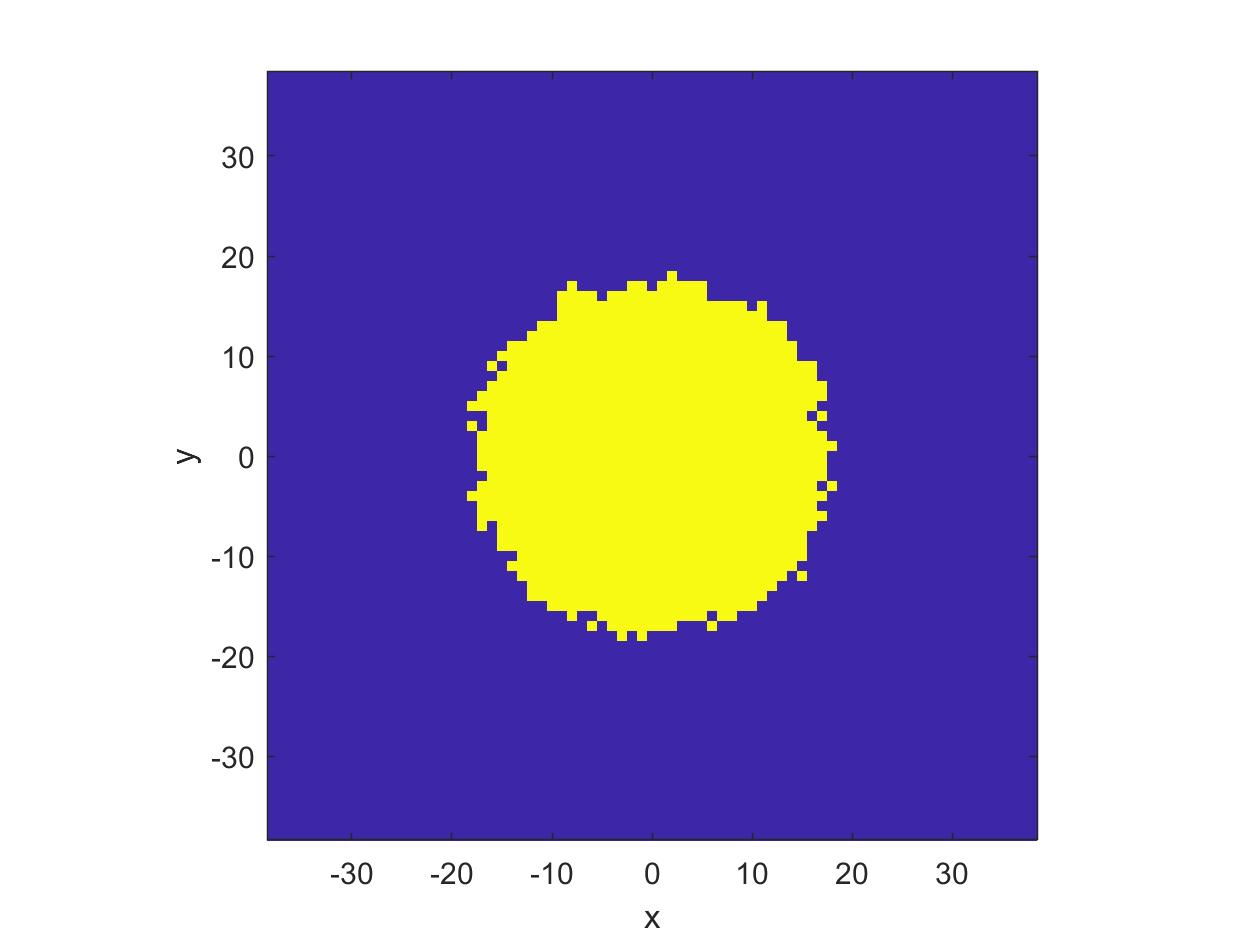
\includegraphics[width=\textwidth]{8direct_Npart1000_3suW11T}
		\caption{\texttt{Npart = 1000}}
		\label{8direct_Npart1000_3suW11T}
	\end{subfigure}
	\begin{subfigure}[b]{0.3\textwidth}
		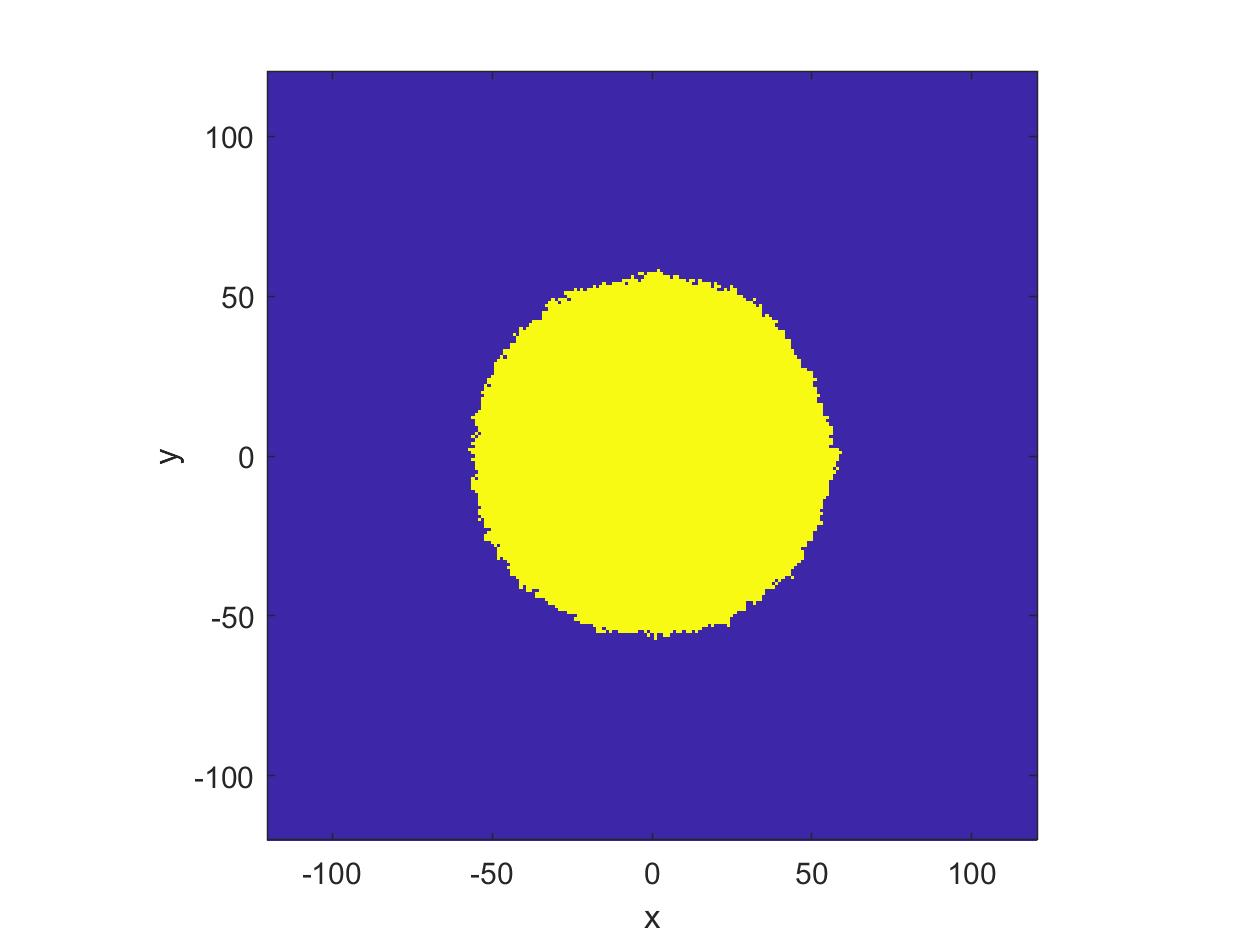
\includegraphics[width=\textwidth]{8direct_Npart10000_3suW11T}
		\caption{\texttt{Npart = 10000}}
		\label{8direct_Npart10000_3suW11T}
	\end{subfigure}
	\caption{IDLA simulation with 8 directions}
	\label{IDLA simulation with 8 directions}
\end{figure}
	



\subsection{Particles move in 4 directions}
My first task is to restrict the motion of direction for each particles which involve in IDLA process. We would like to see if the boundary of the occupied region is still converging to a circle by restricting the particles to choose a random motion in 4 directions. That is, we eliminate the diagonal motion of particles (i.e. upper left, upper right, lower left, lower right). The MATLAB codes to realize this are:

\begin{lstlisting}
    v_dir = [1 0; 0 1; -1 0; 0 -1];
    n_dir = 4;
    
    for i = 1:Npart
      X = [0 0];
      while 1
    
      d = randi(n_dir);
    
      X(1) = X(1) + v_dir(d, 1) + drift(1); 
      X(2) = X(2) + v_dir(d, 2) + drift(2);
      ...
      
\end{lstlisting}

\noindent
Here, we prepare a 4*2 matrix containing 4 vectors which represent four directions that a particle can move along. Then similarly as the case shown in the motion with 8 directions, inside the for loop, we start from the center of the grid quadrant \texttt{[0 0]}. After determining a random number inside a list consisting 1 to 4, we are able to select a vector in the 4*2 matrix and then determine the direction of the particle moves along. The results of the simulation are shown in Fig.1.2.

\begin{figure}[htbp]
	\centering
	\begin{subfigure}[b]{0.3\textwidth}
		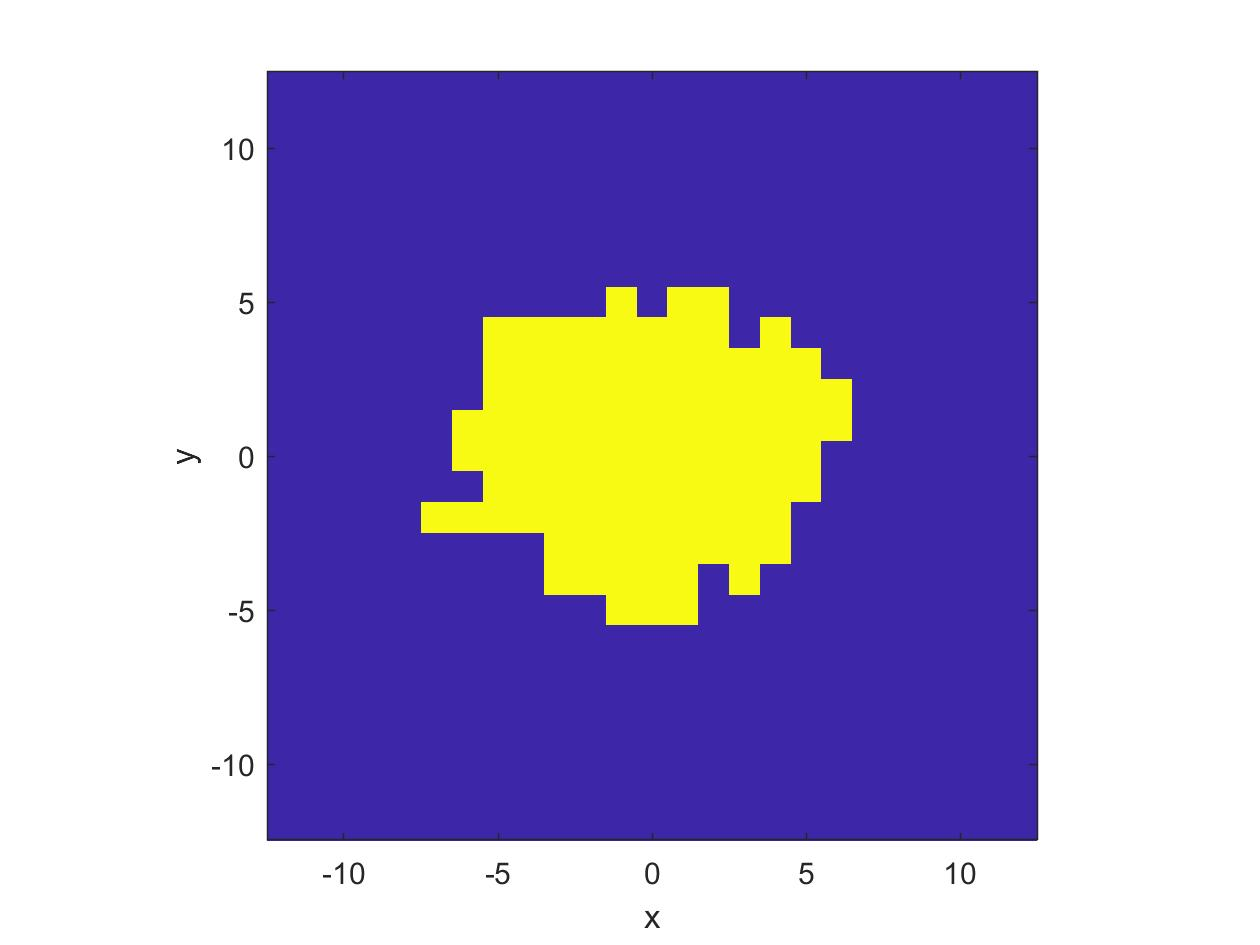
\includegraphics[width=\textwidth]{4direct_Npart100_3suW11T}
		\caption{\texttt{Npart = 100}}
		\label{4direct_Npart100_3suW11T}
	\end{subfigure}
	\begin{subfigure}[b]{0.3\textwidth}
		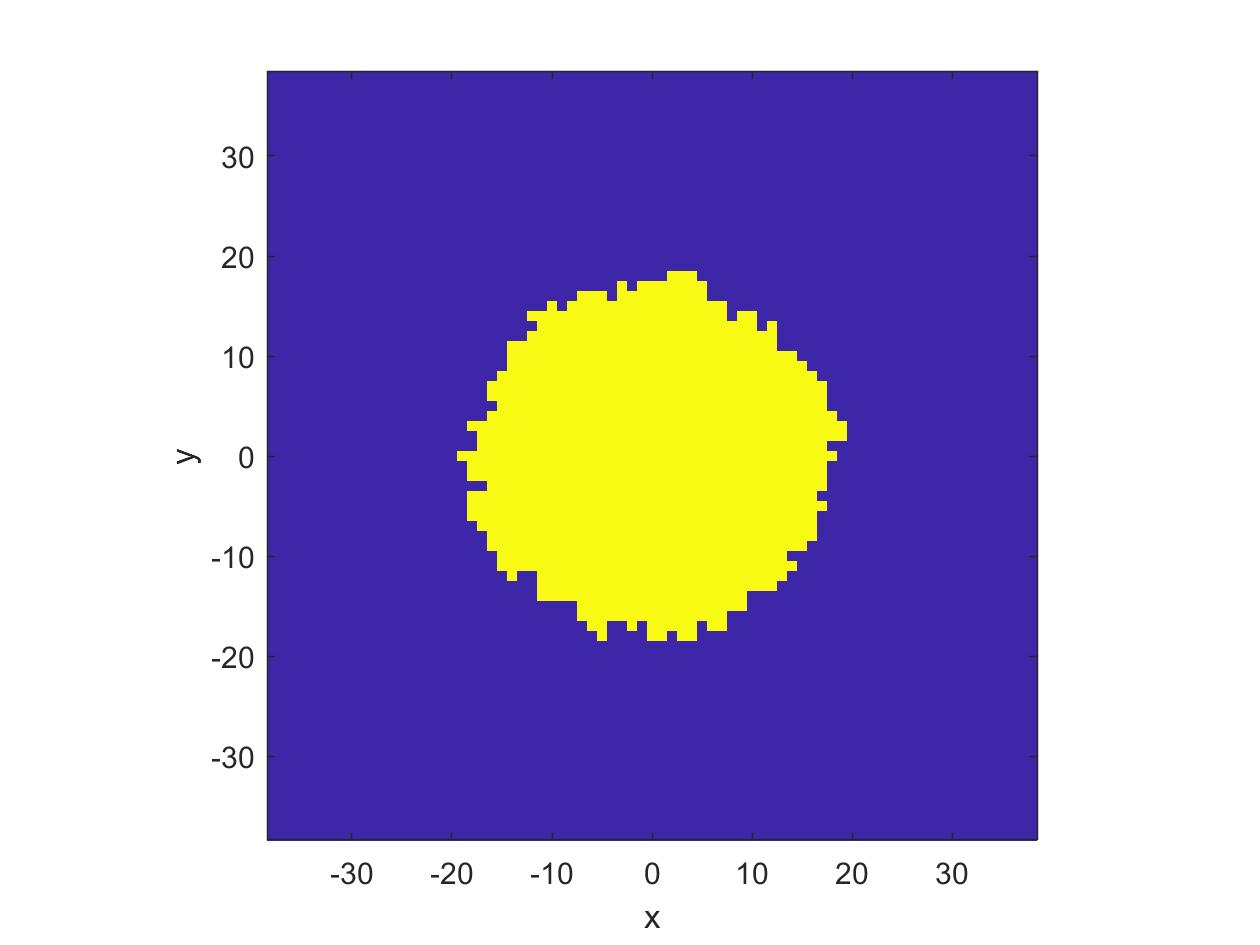
\includegraphics[width=\textwidth]{4direct_Npart1000_3suW11T}
		\caption{\texttt{Npart = 1000}}
		\label{4direct_Npart1000_3suW11T}
	\end{subfigure}
	\begin{subfigure}[b]{0.3\textwidth}
		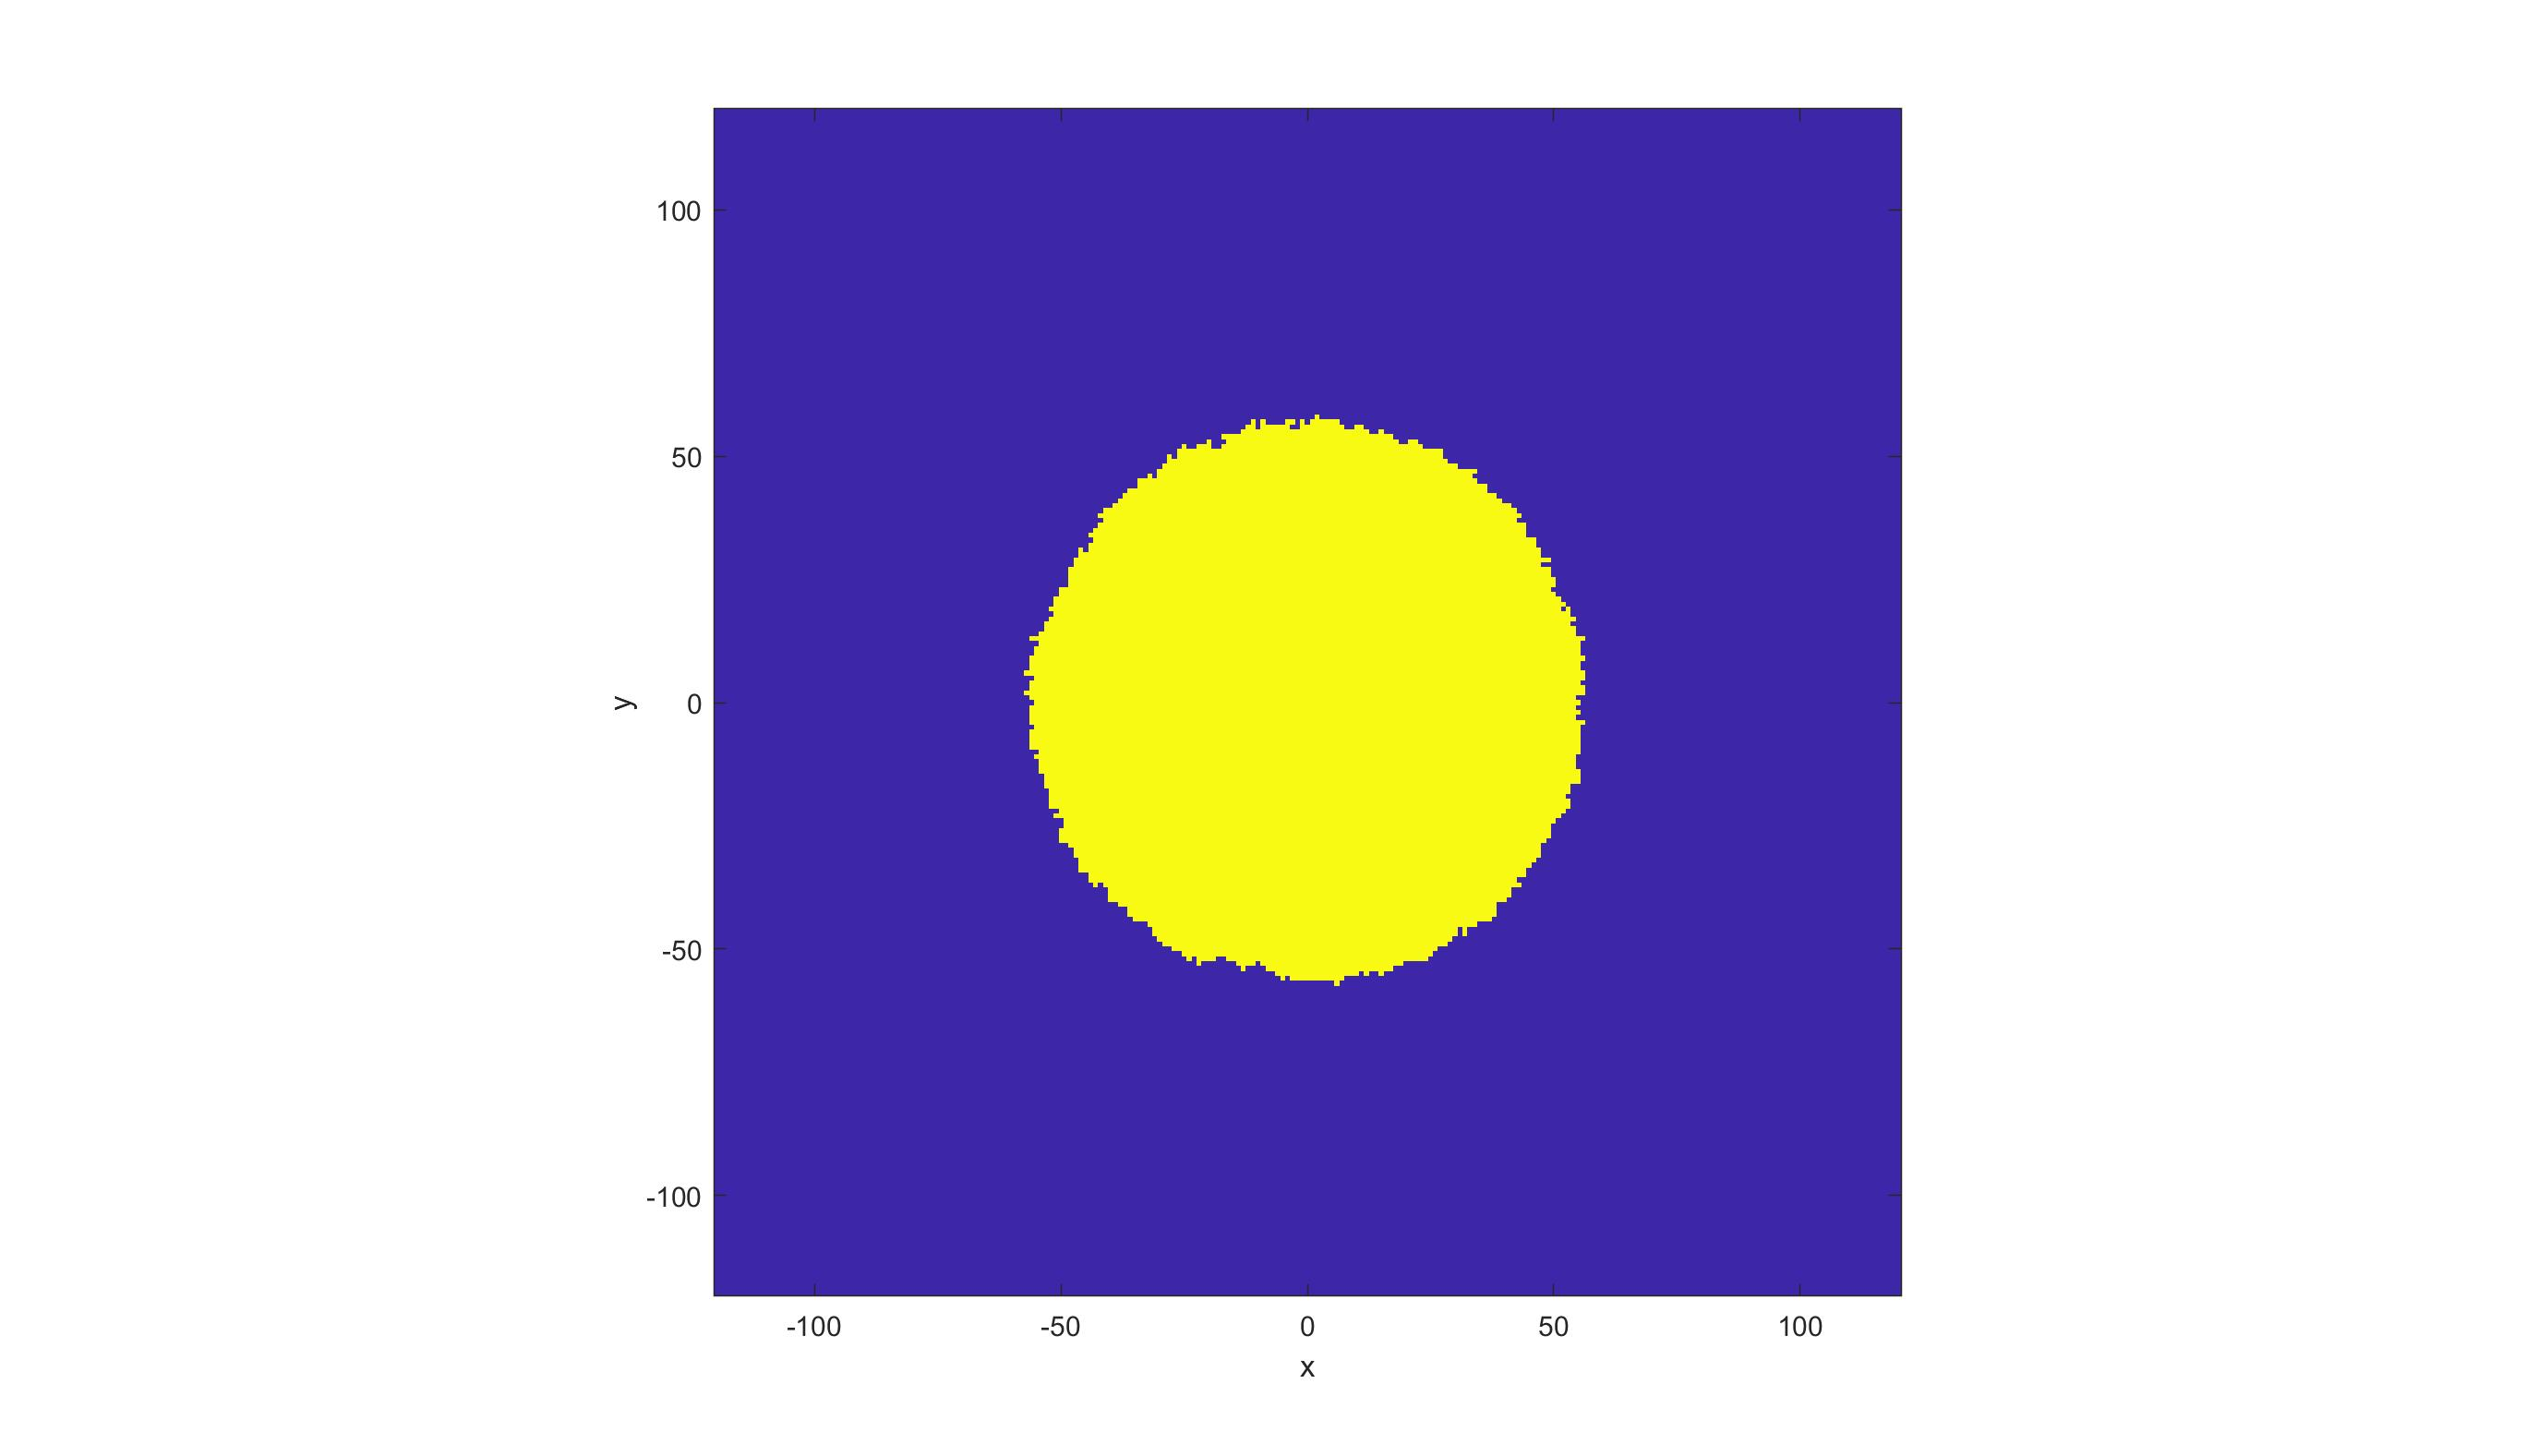
\includegraphics[width=\textwidth]{4direct_Npart10000_3suW11T}
		\caption{\texttt{Npart = 10000}}
		\label{4direct_Npart10000_3suW11T}
	\end{subfigure}
	\caption{IDLA simulation with 4 directions}
	\label{IDLA simulation with 4 directions}
\end{figure}

\noindent
We could then observe that a IDLA simulation also produce a final occupied region which converges to a circle, as the number of particles which participated grows (Fig.1.2).

\subsection{Boundary of the Occupied Region}
From the graph generated by MATLAB codes, we observe that the boundary of the shape constructed by the IDLA process tends to be smooth and to imitate a circle, as the value of \texttt{Npart} (the number of particles) become larger. We want to understand to what extent the shape constructed by the process converges to a circle. We start by selecting out the pixels which constitute the boundary of the occupied region and mainly focus on these pixels. Three different algorithms are tried to remain the boundary only as the IDLA process evolves.

\subsubsection{Three Algorithms to Build the Boundary}

\paragraph{Build entire boundary.}
The idea here is to start from an occupied grid on the boundary (for example, one on the boundary which has the same horizontal coordinate as the center grid), to examine its neighbor occupied grids, to choose the next one which is on the boundary, to examine the neighbors based on this next grid, and hence to find all the grids on the boundary of the occupied region.

(use image maybe?)

\begin{lstlisting}
for k=1:size(bdP,1)  
  if ~(bdP(k,1) == 0 && bdP(k,2) == 0)  
  finish = 0;
  neighb = [bdP(k,1)+1 bdP(k,2); bdP(k,1)-1 bdP(k,2); 
    bdP(k,1) bdP(k,2)+1; bdP(k,1) bdP(k,2)-1; 
    bdP(k,1)+1 bdP(k,2)+1; bdP(k,1)+1 bdP(k,2)-1; 
    bdP(k,1)-1 bdP(k,2)+1; bdP(k,1)-1 bdP(k,2)-1];

    for j=1:8
      if (grid(neighb(j,1), neighb(j,2))==1 && 
      gridB(neighb(j,1), neighb(j,2))==0)  

        if ~((grid(neighb(j,1)+1, neighb(j,2))==1) && 
        (grid(neighb(j,1)-1, neighb(j,2))==1) && 
        (grid(neighb(j,1), neighb(j,2)+1)==1) && 
        (grid(neighb(j,1), neighb(j,2)-1)==1)) 

          bdP = [bdP; neighb(j,1) neighb(j,2)];    
          gridB(neighb(j,1), neighb(j,2))=1;  
          ...
\end{lstlisting}

\noindent
In the first for loop, we prepare the coordinates of all eight neighbors for one particular occupied grid: Since the boundary of the occupied region can be constructed by grids which are only connected diagonally, so to examine the total eight closest grids for one is necessary. If an occupied grid is marked as "1" and an unoccupied one is marked as "0," we can determine the next occupied grid on the boundary by seeing if all its horizontally and vertically connected neighbors are marked as "1."

\paragraph{Build boundary incrementally.} 
This algorithm is designed to examine all the grids on the grid quadrant and select out the grids which construct the boundary only as the occupied region grows. The idea is to come up with a method to tell the difference between the grids inside the region and outside it: the grids which are not on the boundary are surrounded by grids along its four sides, while the grids which are on the boundary have at least one side which does not touch another grid. Hence, as one more particle is added to the process, we could eliminate those which are not considered on the boundary. For example, in Fig.1.3, when the fifth particle is added to the process, we can determine the grid at the center is no longer a grid on the boundary and it should be removed. The MATLAB codes are shown as following: 

\begin{figure}[h]
		\centering
		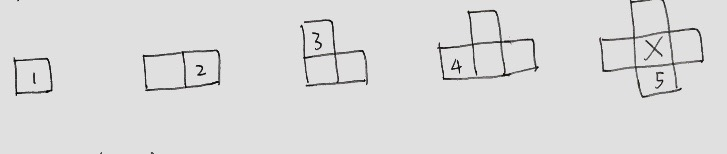
\includegraphics[width=0.7\linewidth]{bdryAlg2}
		\caption{remove a grid which is not considered on the boundary any longer}
		\label{fig:bdryAlg2}
\end{figure}




\begin{lstlisting}
for k = 2:(2*grid0-1)
  for l = 2:(2*grid0-1)
    if grid(k, l) == 1 && grid(k, l+1) == 1 && 
    grid (k, l-1) == 1 && grid (k+1, l) == 1 && 
    grid (k-1, l) == 1
    
      gridB(k, l) = 0; 
      ...
\end{lstlisting}

\noindent
where the grids which are occupied are marked as "1," and those which are not occupied are denoted as "0." By examining if all four neighbors of one grid are marked as "1," we are able to determine whether one grid is considered on the boundary.


\paragraph{Build boundary by Discrete Laplace.}
The third algorithm using Discrete Laplace has the similar idea to the second one. A Discrete Laplace can be written as:

\begin{align} 
(\Delta f)_{i,j} = 4f_{i,j}-f_{i+1,j}- f_{i-1,j}-f_{i,j+1}-f_{i,j-1}
\end{align}

\noindent
Similarly to the second algorithm, the grids which are occupied are marked as "1," and those which are not occupied are denoted as "0." Hence, if $(\Delta f)_{i,j}>0$, the grid with coordinate $(i,j)$ is considered on the boundary. The MATLAB codes can be written as:

\begin{lstlisting}
for k = 2:(2*Ngrid)
  for l = 2:(2*Ngrid)
    delta_f = 4*grid(k, l) - grid(k, l+1) - grid(k, l-1) 
    - grid(k+1, l) - grid(k-1, l);

    if delta_f == 0  
      gridB(k, l) = 0; 
      ...
\end{lstlisting}

In order to see if those three algorithms return the same results regarding the grids on the boundary which are selected out, I also further compare the discretized boundary generated by three algorithms and it turns out they agree with each other.




\subsubsection{The Numerical Standard Deviation}
Consider each grid we selected on the boundary previously with a center at coordinate $(m_i,n_i)$, where $0\leq i\leq N$ and $N$ denotes the total number of particles on the boundary. To determine how the particle occupied region converges to a circle, we can compute a average distance $\overline{d_N}$ based on the distance between the center of each grid on the boundary and the center of the grid quadrant. 

\begin{align} 
\overline{d_N} = \frac{1}{N} \sum_{i=0}^{N-1} (m_i^2+n_i^2)^{\frac{1}{2}}.
\end{align}
 
\noindent
This distance $\overline{d_N}$ can be roughly considered as the radius of a circle $O$, if we could obtain such an $O$ when the number of particles participating in the IDLA process $N \rightarrow \infty$. The numerical value of such a $\overline{d_N}$ can be computed by MATLAB codes. When one more particle is added to the process, a new value of $\overline{d_N}$ would be computed. Hence, we can plot $\overline{d_N}$ versus the number of particle $N$ to see how $\overline{d_N}$ grows then. From Fig 1.4, we see that $\overline{d_N}$ and $N$ are roughly linearly related. We further compute the standard deviation $\sigma_N$, with respect to the particle number $N$

\begin{align} 
\sigma_N = \frac{1}{N} \sum_{i=0}^{N-1} (d_N-\overline{d_N})^{\frac{1}{2}}.
\end{align}

\noindent
The relation of $\sigma_N$ versus $N$ can also be plotted by MATLAB (Fig 1.4). When $N=10000$, $\sigma_N=0.72172$. If the occupied region generated by IDLA process converges to a circle as we expected previously, $\sigma_N$ should be also converging as a smooth function with respect to a large $N$; however, it is hard to see if $\sigma_N$ converges from the plot. We need to examine further.

We denote this $\sigma_N$ as $\sigma_{sim}$, saying that this is the standard deviation given by the whole simulation. It consists of two different errors, the geometric error $\sigma_{geom}$ and the statistical error $\sigma_{stat}$. We would first look at the the geometric error $\sigma_{geom}$, since it helps us understand how big this value this even if we draw a perfect circle on a grid quadrant.

\begin{figure}[h]
	\centering
	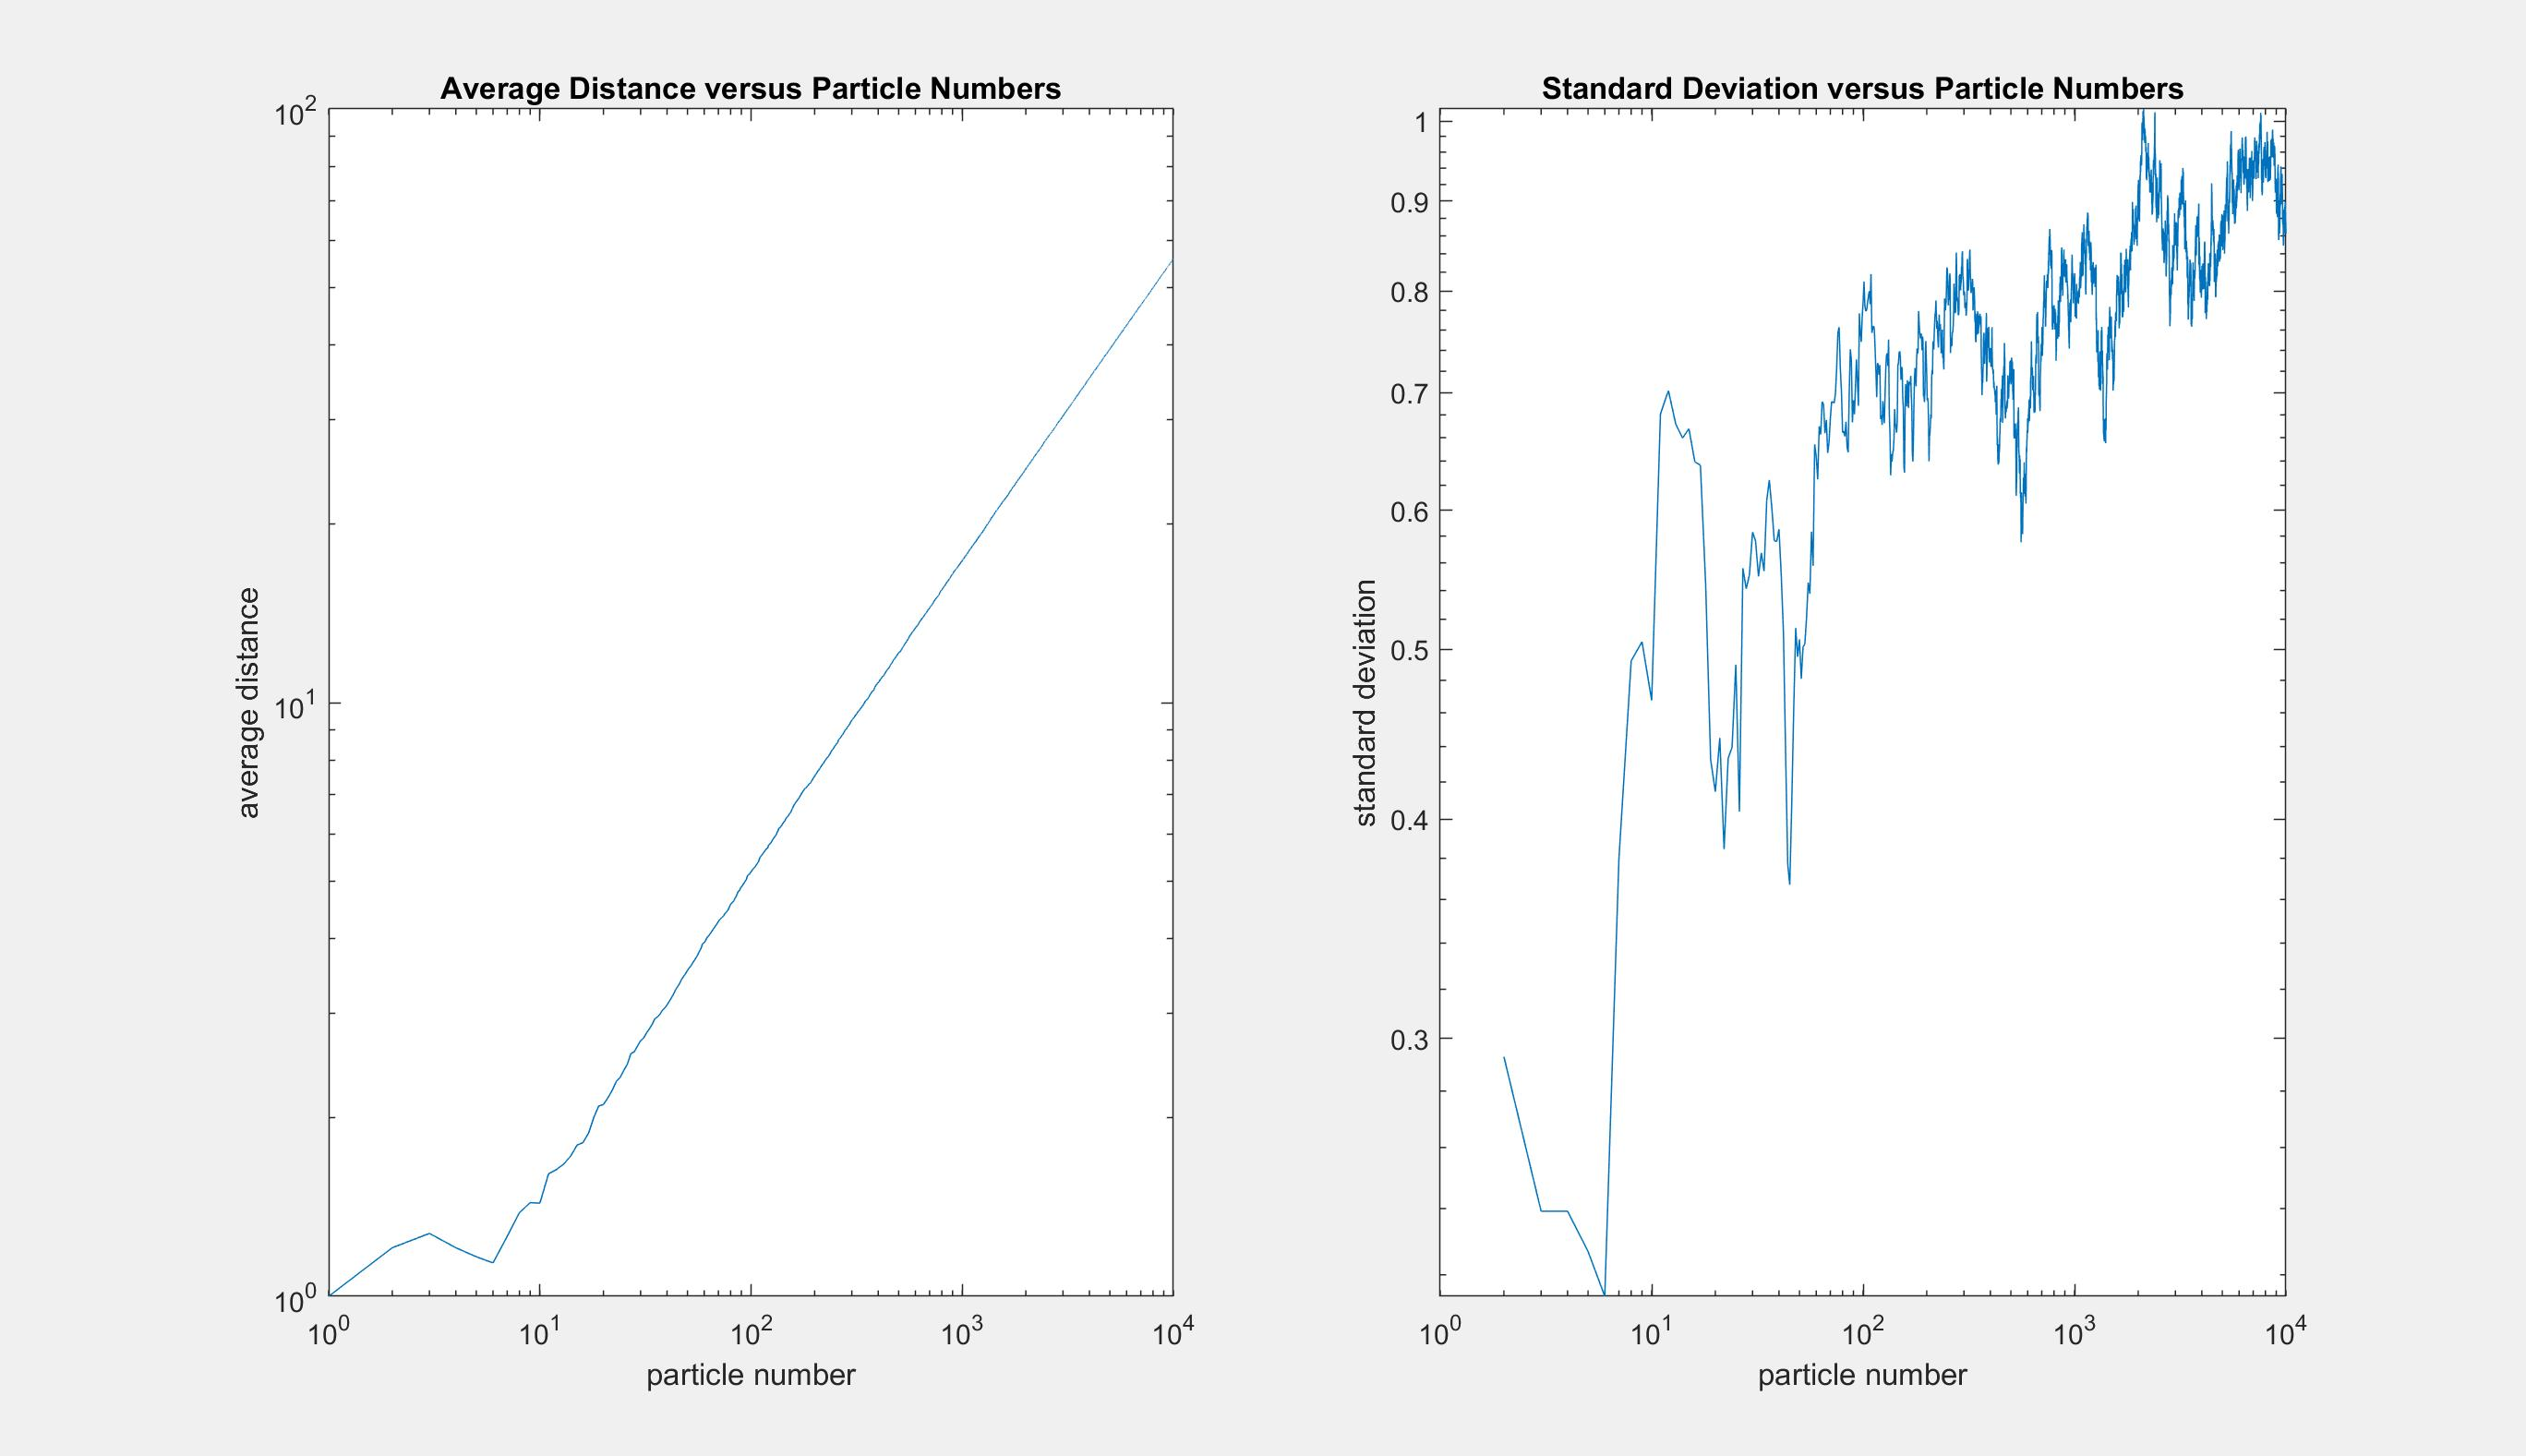
\includegraphics[width=0.7\linewidth]{bdryRandSTD}
	\caption{Average distance versus particle numbers and standard deviation versus particle numbers when \texttt{Npart=10000}.}
	\label{fig:bdryRandSTD}
\end{figure}








\section{The Geometric Error}

The basic setup is given by Professor Thiffeault's handout "On Discretizing a Circle". We consider a grid (a lattice of circle) in the plane with centers at coordinates $p=(m, n)\in\mathbb{Z}^2$. The center of circle drawn locates at the origin $(0,0)$. Take a circle of radius $R$, centered on the origin. A continuous discretization of the circle is an ordered set of distinct pixels 

\begin{align} 
\mathcal{D}_R=(p_{i})_{0 \leq i \leq N-1} = (m_i, n_i)_{0 \leq i \leq N-1},
\end{align}

\noindent
where $m_i$ denotes the horizontal coordinate of the center of a pixel and $n_i$ denotes the vertical one of that.

There are two different ways to construct such a discretized circle. For convenience, we call them \enquote{non-remove} case and \enquote{remove} case.


\subsection{Two Types of Discretized Circle and Their Numerical Standard Deviation}

\subsubsection{The \enquote{Non-remove} Case}


In a "non-remove" case, the pixels $p_i$ is just those which the boundary of the circle centered at $(0,0)$ passes through. The resulted boundary consists of the grids connected horizontally, vertically, and diagonally (Figure 2.1). 

\begin{figure}[htbp]
	\centering
	\begin{subfigure}[b]{0.2\textwidth}
		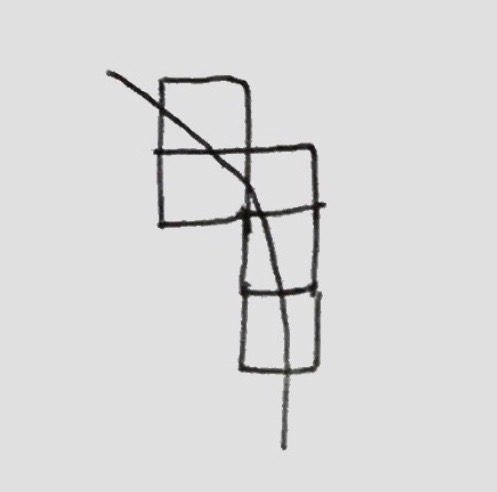
\includegraphics[width=\textwidth]{NonrmvSetup}
		\caption{The \enquote{non-remove} case.}
		\label{NonrmvSetup}
	\end{subfigure}
	\begin{subfigure}[b]{0.2\textwidth}
		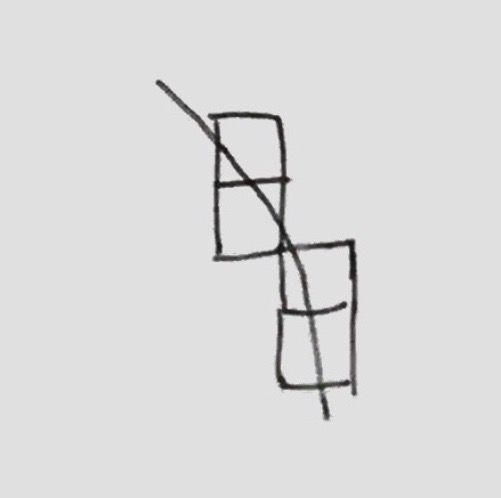
\includegraphics[width=\textwidth]{RmvSetup}
		\caption{The \enquote{remove} case.}
		\label{RmvSetup}
	\end{subfigure}

	\caption{Construct the discretized boundary of \enquote{non-remove} and \enquote{remove} cases}
	\label{Construct the discretized boundary of "non-remove" and "remove" cases}
\end{figure}

The algorithm can also be realized by MATLAB codes. The main idea is to start from a grid on the boundary, and to examine its neighbors and to determine the next grid which could be used to construct the boundary of a circle. We only consider grids for the upper right quarter of the circle; other three discretized quarters would just be the mirror images of the upper right one respect to the horizontal or vertical axises in the center. The final constructed circle is shown in Figure 2.2. We can then compute a numerical standard deviation $\sigma_{geom}$. As an example, given $R=10000$, $\sigma_{geom}=0.3729$.

\begin{figure}[htbp]
	\centering
	\begin{subfigure}[b]{0.6\textwidth}
		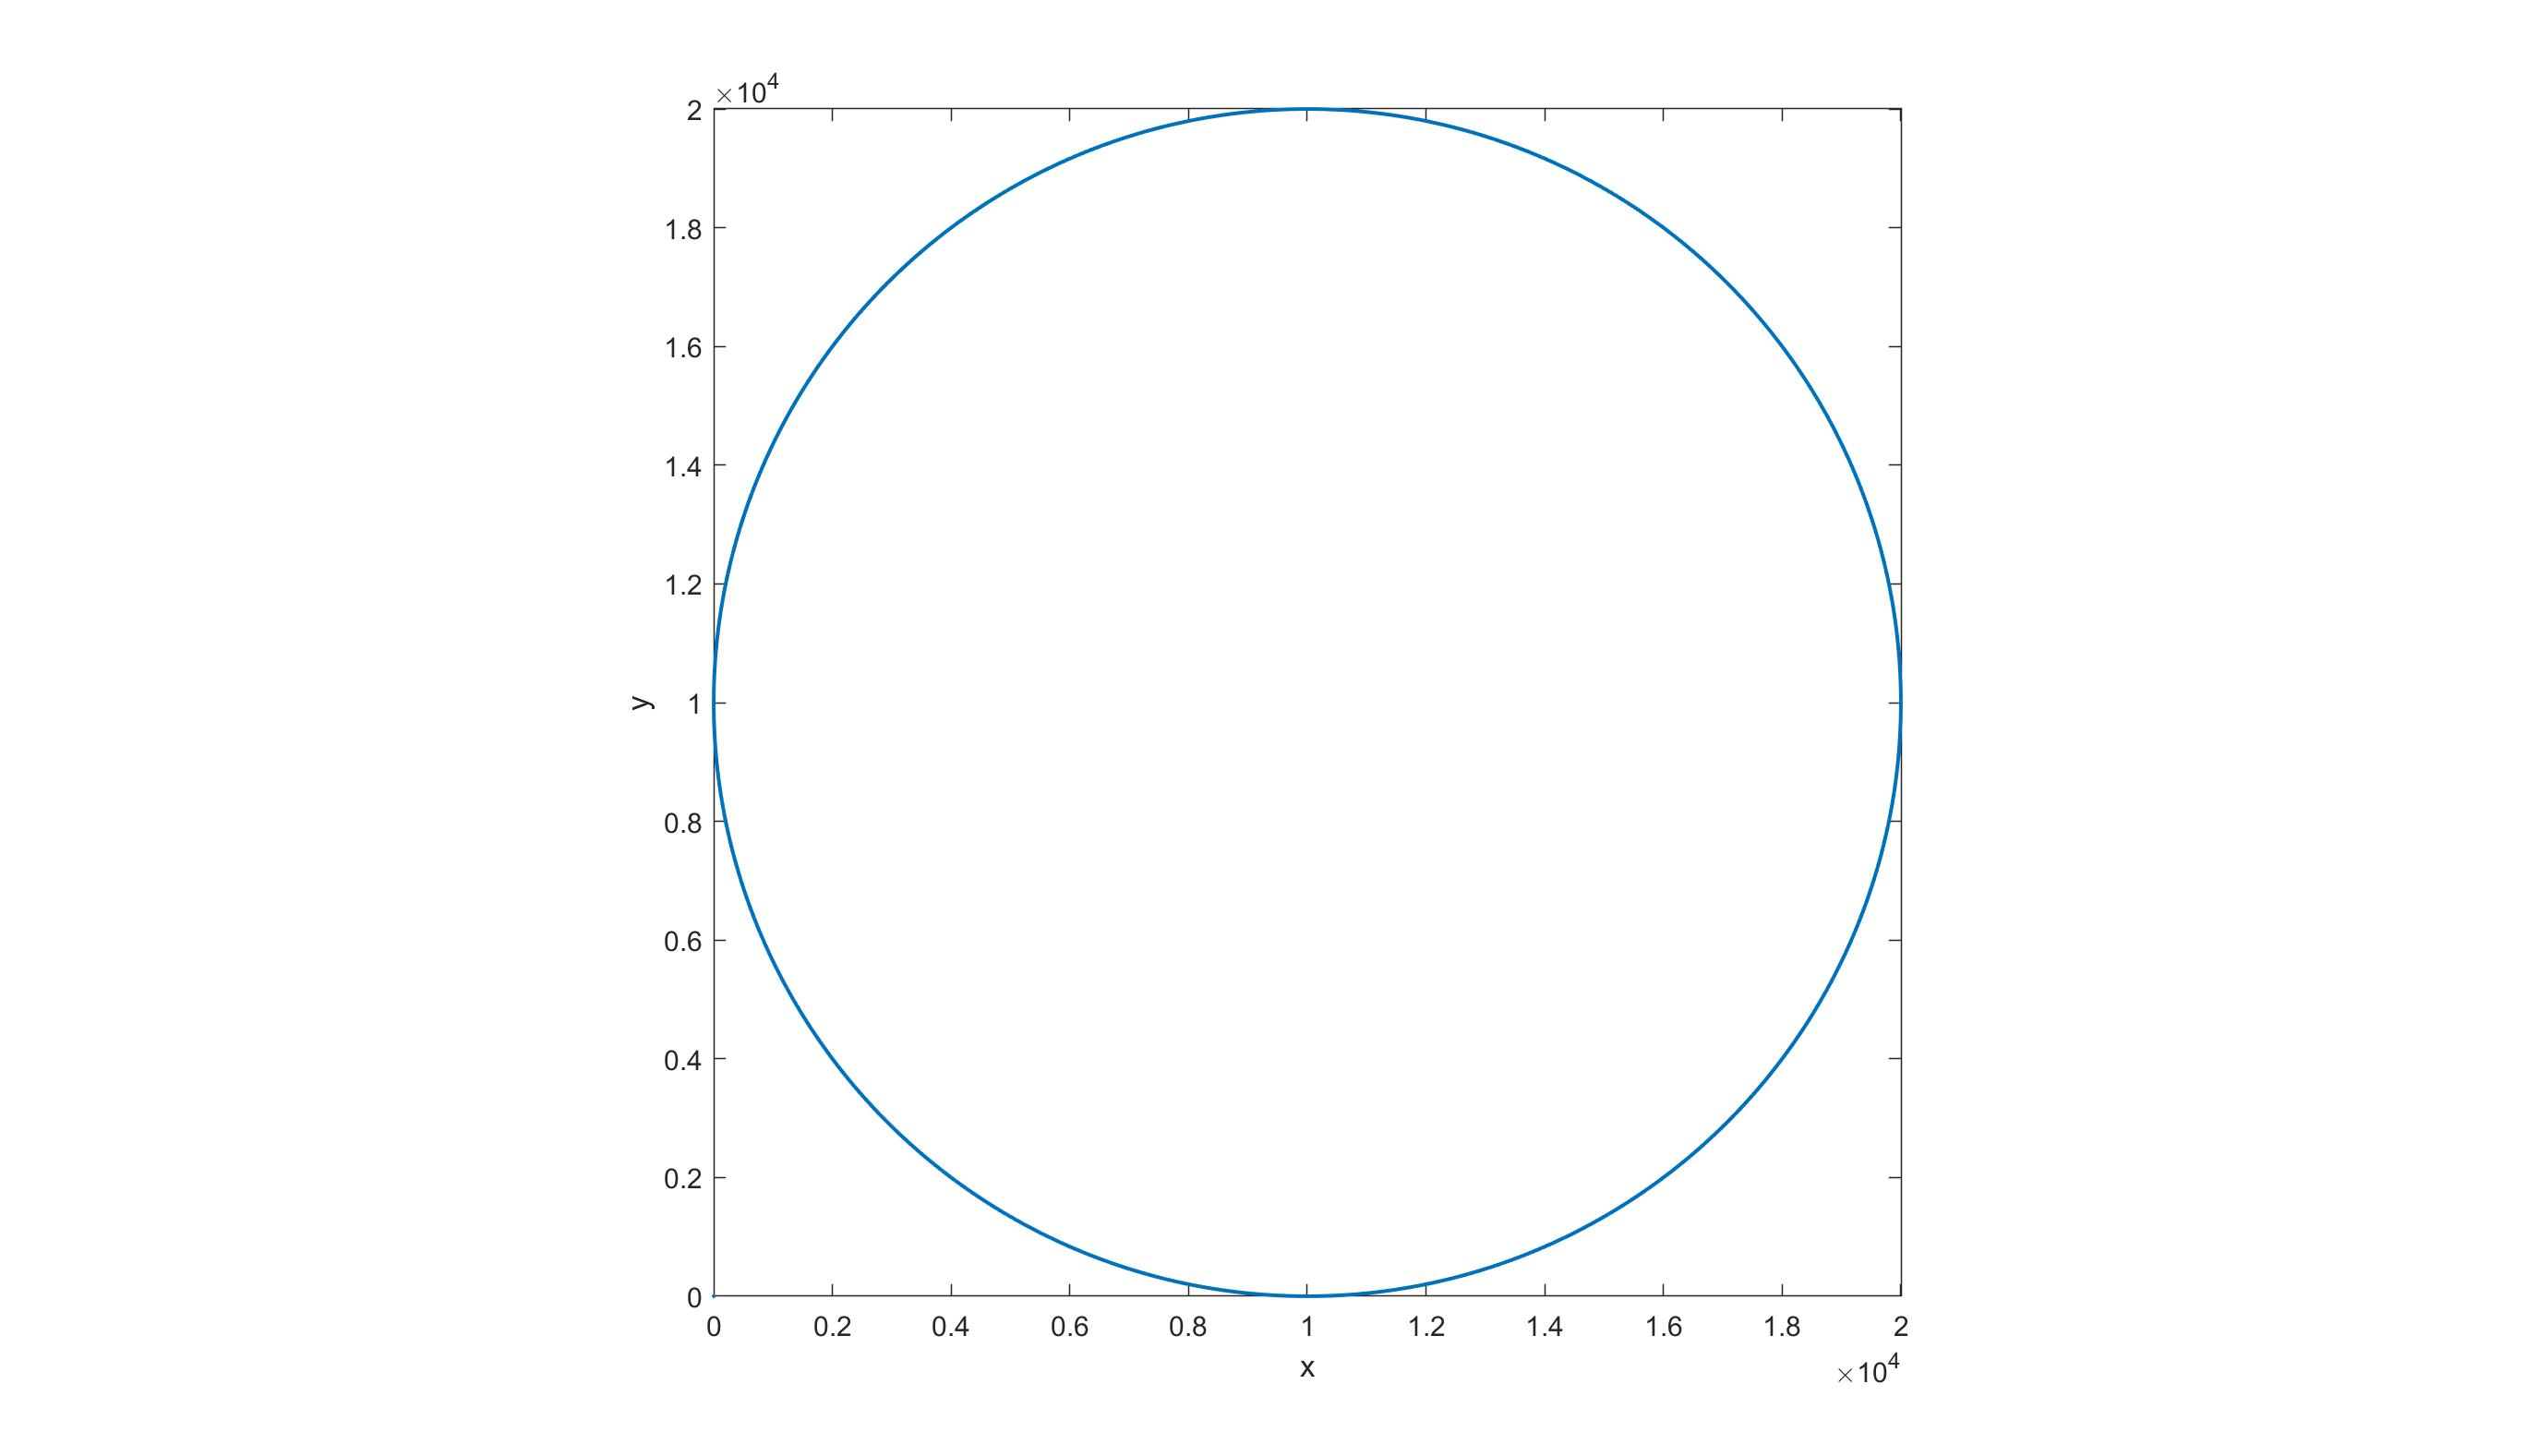
\includegraphics[width=\textwidth]{NonrmvCircle}
		\caption{A \enquote{non-remove} circle.}
		\label{NonrmvCircle}
	\end{subfigure}
	\begin{subfigure}[b]{0.6\textwidth}
		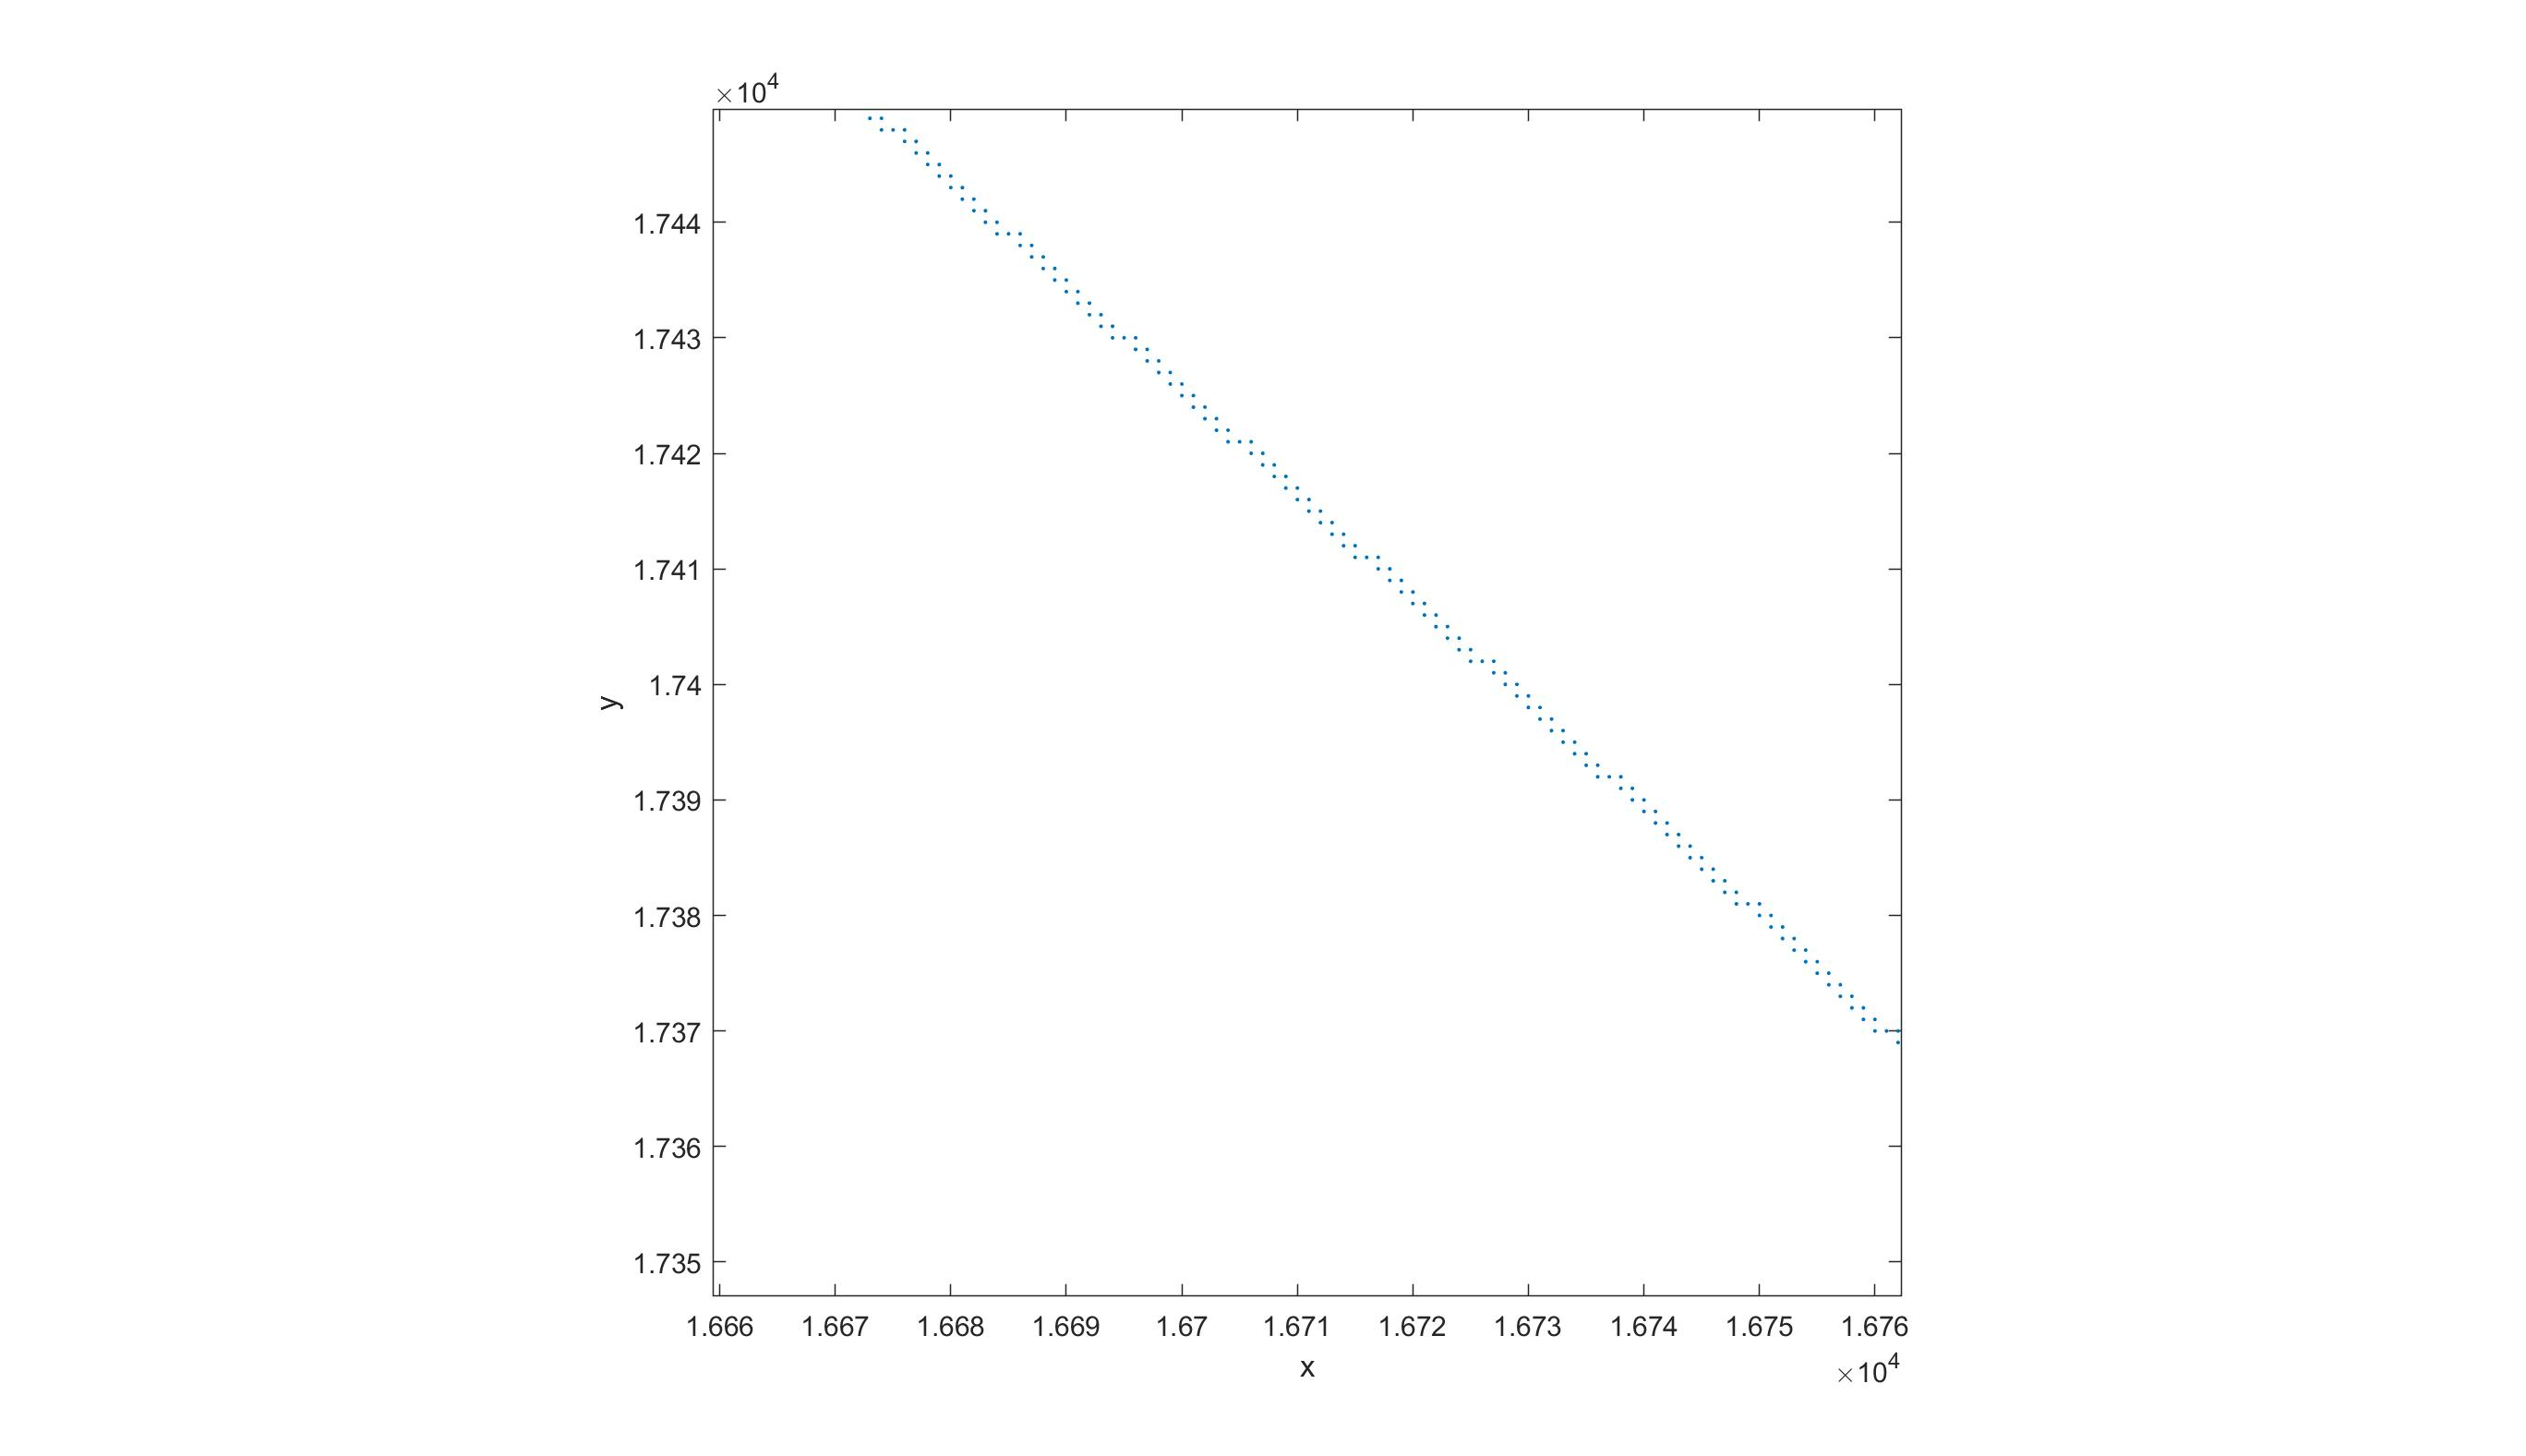
\includegraphics[width=\textwidth]{NonrmvCircleZI}
		\caption{A \enquote{non-remove} circle with $\times 10^4$ zoom in.}
		\label{NonrmvCircleZI}
	\end{subfigure}
	
	\begin{subfigure}[b]{0.6\textwidth}
		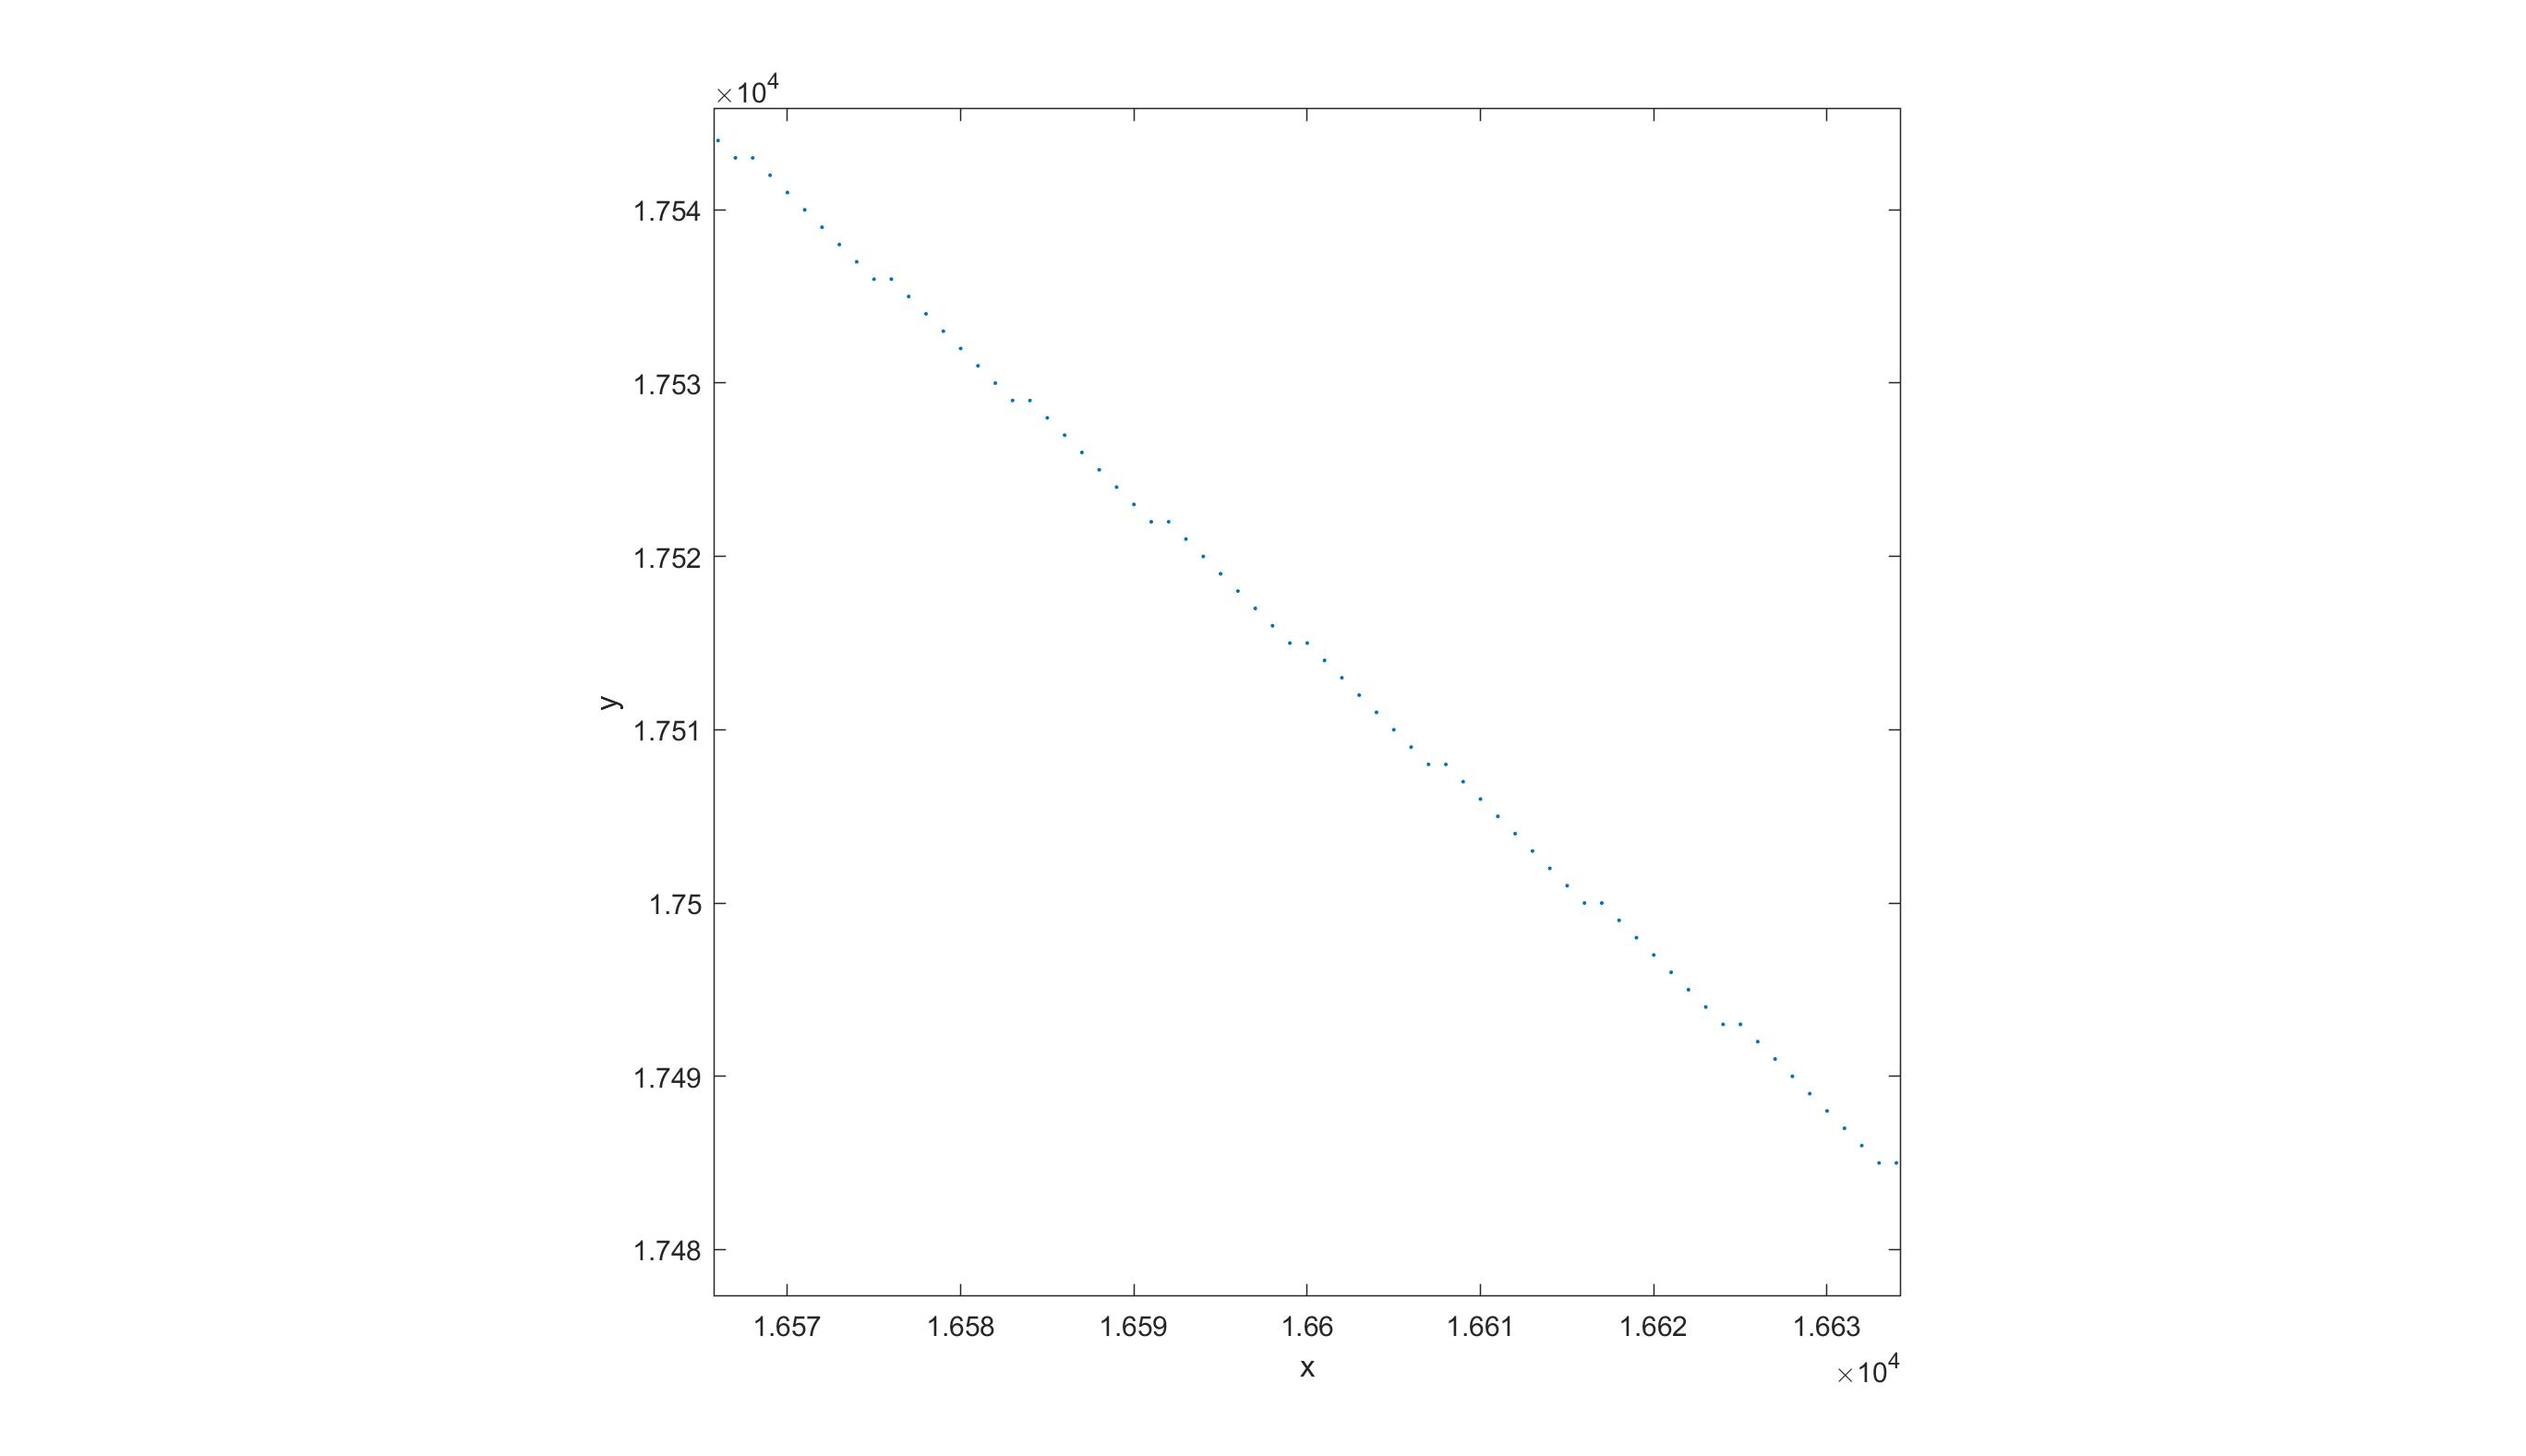
\includegraphics[width=\textwidth]{rmvCircleZI}
		\caption{A \enquote{remove} circle's $\times 10^4$ zoom in.}
		\label{rmvCircleZI}
	\end{subfigure}

	\caption{A \enquote{non-remove} circle, its $\times 10^4$ zoom in, and a \enquote{remove} circle's $\times 10^4$ zoom in. Circle gridpoints rather than square colored grids are used to raise the computation speed. }
	\label{circle and zoom in}
\end{figure}

	
\subsubsection{The \enquote{Remove} Case}

Another ways to construct a discretized consisting of less pixels on the boundary than those in the first algorithm: The boundary of the cirlce might or might not pass through each pixel, but no grids on the boundary can have more than one horizontally or vertical neighbors (?) (Figure 2.1).

The algorithm can be realized by MATLAB codes: The main procedures are similar to those for a \enquote{non-remove} circle; when we examine neighbors of one particular grid, we only remain the neighbor whose center is closest to the boundary of the circle which passes through (Figure 2.2(c)). The numerical standard deviation can be computed: When $R=10000$, $\sigma_{geom}=0.2624$, which is smaller than the value obtained from the first algorithm.

\subsection{The Upper Bound of $L_{2}$ Error of the Discretization}

A derivation of $L_{2}$ Error of the discretization is provided by Professor Thiffeault's handout "On Discretizing a Circle". Once we have $\mathcal{D}_R=(p_{i})_{0 \leq i \leq N-1} = (m_i, n_i)_{0 \leq i \leq N-1}$, we define the average radius of $\mathcal{D}_R$ as


\begin{align} 
\text{Rad} \ \mathcal{D}_R=\frac{1}{N} \sum_{i=0}^{N-1} (m_i^2+n_i^2)^{\frac{1}{2}}.
\end{align}

\noindent
In order for a discretization to be valid, it must converge to the circle in the limit as $R \rightarrow \infty$: (?)

\begin{align} 
\lim_{R \rightarrow \infty} \ \text{Rad} \ \mathcal{D}_R = R.
\end{align}

\noindent
The $L^2$ error can then be written as 

\begin{align} 
\text{Err}_2 \ \mathcal{D}_R=(\frac{1}{N} \sum_{i=0}^{N-1} (m_i^2+n_i^2)-R^2)^{\frac{1}{2}}.
\end{align}


In both algorithm to construct a discretized circle, $\sigma_{geom}$ can be approximated by Err$_2 \ \mathcal{D}_R$ when $R \rightarrow \infty$. Err$_2 \ \mathcal{D}_R$ can also be considered as the distance between the center of each pixel $p_i$ and the boundary of the circle which passes through this pixel. We denote Err$_2 \ \mathcal{D}_R$ as $d$ in this case and denote a small piece of the boundary passing through each circle as $c_i$. Assume that this piece $c_i$ is randomly distributed in each grid; we could then compute the expectation value $\mathbb{E}\ d^2$: Suppose a small region inside a grid with area $dx \times dy$ such that $x$ represents the horizontal coordinate and $y$ represents the vertical one. The probability density function $p(x,y)$ is then given by

\begin{align} 
p(x,y)=\frac{1}{A}=1
\end{align}

\noindent
where $A$ represents the area of one grid and equals to 1. $p(x,y)$ also fulfills $\int_{0}^{1}\int_{0}^{1}p(x,y) \ dx \ dy=1$. Also, with 

\begin{align} 
d^2=(x-\frac{1}{2})^2+(x-\frac{1}{2})^2,
\end{align}

\noindent
the expectation value of $d^2$ can be computed by

\begin{align} 
\mathbb{E}(d^2) = \int_{0}^{1} \int_{0}^{1}f(x,y) \ p(x,y) \ dx \ dy = 2 \  \mathbb{E}(x-\frac{1}{2})^2 = 2 \int_{0}^{1}(x-\frac{1}{2})^2 \cdot 1 \ dx = \frac{1}{6}.
\end{align}

\noindent
Thus, if the small piece is randomly distributed, the expectation value $\mathbb{E}\ d^2 \approx 0.1667$. 

For both the \enquote{non-remove} and \enquote{remove} cases, a analytical upper bound can be found for $d^2$, which approximately equal to $\sigma_{geom}^2$ when $R \rightarrow \infty$. $\sigma_{geom}^2 \leq \frac{1}{2} \approx 0.5$ and then $\sigma_{geom} \leq 0.7071$. Our next task is to lower down this upper bound and obtain a new bound which is as close to $0.1667$ as possible. We firstly sort pixels into 4 different types as following to lower the upper bound of $d^2$.

\subsubsection{Sort Pixels into 4 Different Types}
According to the ways that the boundary of the circle passes through each pixel, we can sort $N$ pixels into 4 different types for the upper right quarter of the circle (other three quarters would just be the mirror images of the upper right one with respect to different axises of symmetry). As the algorithm provided above, the center of each pixel is represented by $(m_i, n_i)$. The boundary of the circle passing by would have 2 different intersections with a pixel $p_i$. Hence, the four different type of grids can be given by the inequalities restricting the coordinates $(x,y)$ of the intersections. For example, the intersection point A in the first kind of pixel is provided by  

\begin{align} 
x=m_i-\frac{1}{2}; \ n_i-\frac{1}{2}\leq y \leq n_i-\frac{1}{2}, \ \text{where} \ y=\sqrt{R^2-(m_i-\frac{1}{2})^2};
\end{align}

\begin{figure}[h]
	\centering
	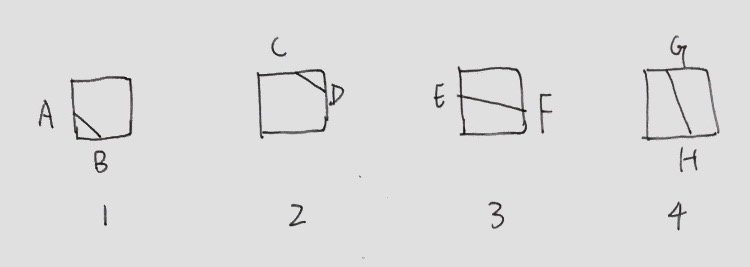
\includegraphics[width=0.5\linewidth]{4ty}
	\caption{Sort pixels into 4 different types}
	\label{fig:4ty}
\end{figure}

\noindent
We guess that these four different types of pixels might hold different upper bounds of $L^2$ error. Hence, by weighing four different values of upper bound correctly with respect to the fractions of these types of pixels, we might be able to obtain a smaller upper bound for $\sigma_{geom}$. With MATLAB codes, when $R=10000$, the numerical fraction of the four different type of pixels in the first quarter for a "non-remove" case are 

\begin{align} 
\text{fraction of type 1}=0.29291; \\
\text{fraction of type 2}=0.29286; \\
\text{fraction of type 3}=0.20711; \\
\text{fraction of type 4}=0.20711; 
\end{align}

\noindent
For a "remove" case, this would be
\begin{align} 
\text{fraction of type 1}=0.20522; \\
\text{fraction of type 2}=0.20897; \\
\text{fraction of type 3}=0.29291; \\
\text{fraction of type 4}=0.29291; 
\end{align}

\paragraph{A derivation for upper bound of the error.}
$Q_{m,n}$ denotes the distance between the center of the circle and the center of one pixel (corresponding to $\overline{d_N}$ defined in IDLA process); R is the radius of the circle.

\begin{align} 
|Q_{m,n}-R| \leq \frac{1}{\sqrt{2}} 
\end{align}

\noindent
We then define a $D(a,b)$ such that

\begin{align} 
D(a,b) = \sqrt{a^2+b^2} 
\end{align}

\noindent
where $D(a,b)$ gives the values which specify a particular corner of pixels we are looking at. For example, for the lower left corner of a grid in the first type, $D(a,b)=D(-\frac{1}{2},-\frac{1}{2})$. As an example, We can then compute a generalized difference $D(m-\frac{1}{2}, n-\frac{1}{2})-D(m,n)$ such that

\begin{align} 
|D(m+a, n+b)-D(m,n)|\leq R-\sqrt{m^2+n^2} 
\end{align}

\noindent
where $m=Q_{m,n}\cos \theta_{m,n}$ and $n=Q_{m,n}\sin \theta_{m,n}$. Substitute those two expressions into (2.12), we obtain

\begin{align} 
\sqrt{(Q_{m,n}\cos \theta_{m,n}+a)^2+(Q_{m,n}\sin \theta_{m,n} +b)^2}-Q \\
=Q(\sqrt{1+\frac{2}{Q}(a\cos \theta+b\sin \theta)+\frac{a^2+b^2}{Q^2}}-1)
\end{align}

\noindent
By Taylor expansion, we have 

\begin{align} 
D(m-\frac{1}{2}, n-\frac{1}{2})-D(m,n) = a\cos \theta +b\sin \theta + \mathcal{O}(Q^{-1}) \leq R-Q_{m,n}
\end{align}

\noindent
Hence, (?)
\begin{align} 
Q_{m,n}-R \leq D_{m,n}-D_{m-\frac{1}{2},n-\frac{1}{2}} \leq \frac{1}{2}(\cos \theta_{m,n}+\sin \theta_{m,n})+\mathcal{O}(R^-1) \\
\Rightarrow \ -\frac{1}{\sqrt{2}R} \leq \frac{Q_{m,n}}{R}-1 \leq \frac{1}{\sqrt{2}R}
\end{align}

\noindent 
By the same procedures, we can obtain the inequality (2.16) with other three different $D(a,b)$. According to the definition of variance $\sigma^2$, we have 
\begin{align} 
\sigma_{m,n}^2 = \mathbb{E}[Q_{m,n}^2-R^2]
\end{align}

\noindent
Square both sides of (2.16),
\begin{align} 
\frac{Q_{m,n}^2}{R^2}-\frac{2\ Q_{m,n}}{R}+1 \leq \frac{1}{2R^2} \\ \Rightarrow \frac{\mathbb{E}[Q_{m,n}^2]}{R^2}-\frac{2\ \mathbb{E}[Q_{m,n}]}{R}+1 \leq \frac{1}{2R^2} \\
\Rightarrow \frac{\mathbb{E}[Q_{m,n}^2]}{R^2}-1 \leq \frac{1}{2R^2} \\
\Rightarrow \sigma_{m,n}^2 \leq \frac{1}{2} \approx 0.5
\end{align}

\noindent
Hence, $\sigma_{geom} \leq 0.7071$. The upper bound is still the same as we speculate previously. We need a further improvement.

\subsubsection{An Observation of the Relation between the Fraction of Each Type of Pixels and Multiples of $R$}

This is an observation from examining the numerical values of a particular multiple of radius $R$ and the fraction of each type of pixels. The fraction of each type of pixels is listed in the previous section. We shall look at the geometry of a quarter itself. In Figure.., segment $CD$ is perpendicular to segment $OA$, where $O$ is the center of the circle. We obtain $OD=\frac{R}{\sqrt{2}}$ and $AD=R(1-\frac{1}{\sqrt{2}}) \approx 0.29289R$, where $R$ is the radius of the circle.

\begin{figure}[h]
	\centering
	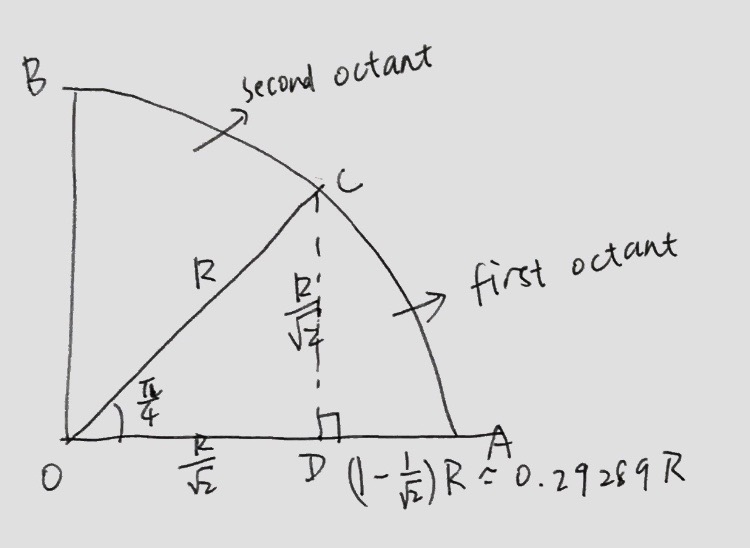
\includegraphics[width=0.4\linewidth]{4tyMultR}
	\caption{The geometry of the upper right quarter and the first octant.}
	\label{fig:4tyMultR}
\end{figure}

\noindent
To construct the relation, we start by examining how each type of grids functions to help the boundary grows from $A$ to $C$. For a \enquote{non-remove} case, the vertically coordinate increases for each pixel; if $R$ is very large, the total increment is approximately $\frac{R}{\sqrt{2}}$. The horizontal coordinate decreases by $R(1-\frac{1}{\sqrt{2}})$ in total. We will only look at the pixels in the first octant since the second octant is just the mirror image of the first one; hence, we just need to consider type 1, 2, and 4, because type 3 would not appear in the first octant. The fractions ($R=10000$) for each type in the first octant are given by 
\begin{align} 
\text{fraction of type 1} = 0.2929;\\
\text{fraction of type 2} = 0.2929;\\
\text{fraction of type 4} = 0.4142;
\end{align}

\noindent
Type 1 and 4 result in vertical increments by 1 pixel; type 2 results in horizontal decrement by 1 pixel. Hence, in the first octant, 
\begin{align} 
\text{number of type 1 and 4}=\frac{R}{\sqrt{2}} \approx 0.70711R;\\
\text{number of type 2}=R(1-\frac{1}{\sqrt{2}}) \approx 0.29289R;
\end{align}

\noindent
Hence, when $R \rightarrow \infty$, multiples of $R$ help determine the fractions of each type of grids. 



For a \enquote{remove} case, from Figure 2.4, we observe that the numerical value represents segment AD might relate with the fraction of type 3 and 4 in a \enquote{remove} case given by (2.16). However, the same method used to derive a relation does not apply to a \enquote{remove} case, since now how each type of grids contributes to a particular increment or decrement is no longer clear. Thus, we need to sort grids in a more specific way. 



\subsubsection{Sort Pixels into 6 Different Types}

\begin{figure}[h]
	\centering
	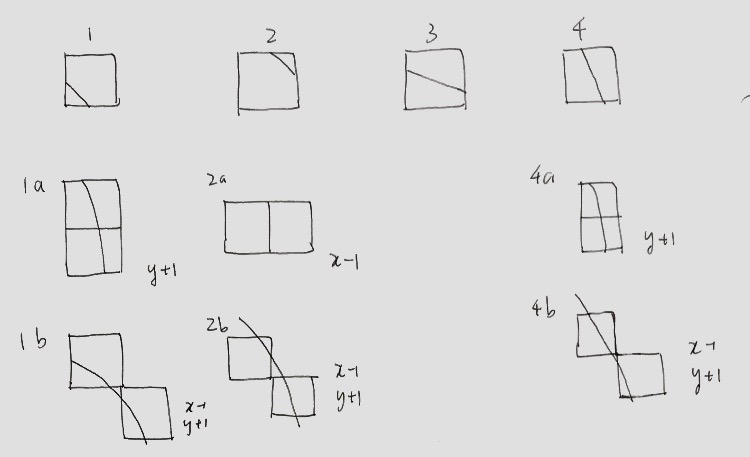
\includegraphics[width=0.5\linewidth]{6ty}
	\caption{Sort pixels into 6 different types.}
	\label{fig:6ty}
\end{figure}

Instead of just sorting pixels into 4 types, we sort those in the first octant into 6 types now, in order to examine more on their functions which cause increments and decrements. Thus, how each type of pixels causes increment or decrement is determined. If we denote the total horizontal decrement as $\delta x$ and the total vertical increment as $\delta y$, then

\begin{align} 
\Delta x \approx n_{1b}+n_{2a}+n_{2b}+n_{4b} \\
\Delta y \approx n_{1b}+n_{1a}+n_{2b}+n_{4a}+n_{4b}
\end{align}

\noindent
where $n_{m}$ gives the number of one type of pixels shown in the first octant. As we show previously, $\Delta x=(1-\frac{1}{\sqrt{2}})R$ and $\Delta y=\frac{R}{\sqrt{2}}$. Substitute these two into the previous equations and simplify, we get

\begin{align} 
n_{4a}+n_{1a}-n_{2a} \approx (\sqrt{2}-1)R
\end{align}

\noindent
To examine the number of type 4, we modify () by constructing a $n_{4a}+n_{4b}$ term on the left hand side

\begin{align} 
n_{4a}+n_{4b} \approx (\sqrt{2}-1)R+(n_{4b}-n_{1a})+n_{2a}
\end{align}

\noindent
$n_{2a}=0$ for the first octant. Also, since every time a 4b type appears, a 1a types appears before it; similarly, when a 1a type shows, a 4b type also shows as its previous pixel. Hence, we have $n_{4b}-n_{1a}=0$. Then we just leave with $n_{4} \approx (\sqrt{2}-1)R$. The total grids in the first octant $n_{total}$ is just $\frac{2R}{\sqrt{2}}$. The fraction of type 4 in the upper right quarter is

\begin{align} 
\frac{n_{4}}{n_{total}} = \frac{(\sqrt{2}-1)R}{\frac{2R}{\sqrt{2}}} = 1-\frac{1}{\sqrt{2}}.
\end{align}

\noindent
Hence, when $R \rightarrow \infty$, fraction of type 4 is just $1-\frac{1}{\sqrt{2}}$. The upper bound of error of type 3 and 4 pixels is $\frac{1}{2}$. Say $p_x$ is the fraction for one kind of pixels; we can weigh a smaller upper bound of $d^2$ by 

\begin{align} 
d^2 \leq p_1 \ (\frac{2}{\sqrt{2}})^2 + p_2 \ (\frac{2}{\sqrt{2}})^2 + p_3 \ (\frac{1}{2})^2 + p_4 \ (\frac{1}{2})^2 \\
= (\sqrt{2}-1) \times (\frac{2}{\sqrt{2}})^2 + (1-\frac{1}{\sqrt{2}}) \times (\frac{1}{2})^2 + (1-\frac{1}{\sqrt{2}}) \times (\frac{1}{2})^2 \\
\approx 0.25
\end{align}

(reference?)

\end{document}